%&pdflatex
\documentclass[12pt,a4paper]{report}
%%\documentclass[12pt,a4paper,twoside,openright,fleqn,MSc]{cusatmscthesis}
\renewcommand{\baselinestretch}{1.15}

\usepackage{dcolumn}
%\newcolumntype{.}{D{.}{.}{-1}}
\usepackage{bm}
\usepackage[colorlinks = true,
linkcolor = red,
urlcolor  = blue,
citecolor = blue]{hyperref}
\usepackage{braket}
\usepackage{graphicx,epsfig,color,subfigure,sidecap,float}
\usepackage{amsmath}
\usepackage{lipsum}
\usepackage{wrapfig}
\usepackage[paperwidth=210mm,paperheight=297mm,centering,hmargin=3cm,vmargin=2.5cm]{geometry}
\usepackage{tcolorbox}
\setlength{\parskip}{1em}
%\usepackage{natbib}
%\usepackage{mathpazo}
%\usepackage{chancery}
%\usepackage{bookman}
%\usepackage{newcent}
%\usepackage{charter}

%\usepackage[scaled=.9]{helvet}
%\usepackage{avant}
%\renewcommand{\familydefault}{\sfdefault}

%%\fontfamily{pzc}\fontsize{10}{12pt}\selectfont

%+Make Index
%\usepackage{makeidx}
%\makeindex
%-Make Index
\bibliographystyle{unsrt}
\usepackage{amssymb}
\usepackage{amstext}
\usepackage{amsmath}
\usepackage{graphicx}
\usepackage{makeidx}
\makeindex

% Title Page
\title{
	\huge Simulating Neutrino Oscillations in a Quantum Computer}
	\vspace{0.5cm}
\author{\large Navaneeth Krishnan M\\
	\small CUSAT, India.}

\begin{document}
\maketitle
\pagebreak	

\chapter{Introduction}
\emph{“ Can physics be simulated by a universal computer? [...] the physical world is quantum mechanical, and therefore the proper problem is the simulation of quantum physics [...] the full description of quantum mechanics for a large a system with R particles [...] has too many variables, it cannot be simulated with a normal computer with a number of elements proportional to R [ ... but it can be simulated with ] quantum computer elements. [...] Can a quantum system be probabilistically simulated by a classical (probabilistic, I’d assume) universal computer? [...] If you take the computer to be the classical kind I’ve described so far [..] the answer is certainly, No! “} 
\begin{flushright}
-Richard P Feynman \cite{feynman82}\cite{nielsen}
\end{flushright}


The primary aim of any sort of simulation is to solve the differential equation that governs the dynamics of the system. One of the most simple example of such an equation is the Newtons equation of motion,
\begin{equation}
m\frac{d^{2}x}{dx} = F
\end{equation}
Generally, the initial state of the system would be input to the problem. Using simulations, one aims to predict the state of the system at a later time or position. The first step in doing any simulation is the encoding of initial state digitally, which more often involves some approximation. Then one has to discretize the dynamical differential equation in space and time. Discretization should be done in such a way that the iterative application of a procedure should evolve the state from initial to final conditions. The accuracy of output state predicted by the simulator depends upon discretization length. Theoretically, as the length of discretization decreases the result would be more accurate. But while computing we need to take into consideration of other sorts of errors that can happen while decreasing the discretization length and often have to find an optimum value. Now, Why this approach works?. This works because the error in is such an approach is bounded and not considerably grows as the number of iterations increases. Further, only those system that can be efficiently described can be simulated efficiently. Thus there are systems where such an approach fails.
en it comes to the question of whether we can simulate a quantum system using a classical simulator, the short answer is yes. But it should be noted that often such simulations are inefficient and fail when the number of particles in the system is very high.  When we analyse the problem of simulating a quantum system, for most of the simple quantum systems, the evolution is given by the time-independent Schrodinger equation. 
\begin{equation}
i\hbar \frac{d}{dt}\ket{\psi} = \hat{H} \ket{\psi}
\end{equation}
On the position basis, the above equation will be 
\begin{equation}
i\hbar\frac{\partial}{\partial t}\psi(x)= \left[ -\frac{\partial^{2}}{\partial x^{2}}+V(x)\right] \psi(x)
\end{equation}
Where $\braket{x|\psi} = \psi(x)$.
Now, assume that we wish to simulate a simple two-level system (Qubit) that obeys the above time-independent Schrodinger equation. For such as system, we have to solve two differential equation to simulate it.If it is a two-qubit system then there would be four equations and so on. Thus, a general system of n qubits $2^{n}$ differential equations must be solved to simulate it. This exponential explosion in the equation is unavoidable unless we employ some approximate methods like Monte Carlo methods\cite{monte} which considerably reduce the number of equations. Such classical stochastic methods would allow us to evaluate the phase-space integrals of many-body quantum systems in polynomial time. But these methods are efficient while the function being integrated does not change its sign. Thus while using such methods, sampling of the function is done in a relatively small number of points. For systems like fermionic or frustrated systems, the integrals encounter the problem of sampling with non-positive semi-definite functions (referred to as negative sign problem\cite{troyer} \cite{georgescu} ) which cause an exponential increase in computation time as the number of particles increases. Thus in such systems, Monte Carlo methods are shown to be inefficient. Other than Monte Carlo methods, there are methods like Density Functional Theory (DFT) \cite{dft}, mean-field theories, Green function-based methods, many-body perturbation theories \cite{mbpt} etc. These methods also have its own limitations.

Richard P Feynman was one of the persons who put forward a solution to this problem. He said that \emph{“ Let the computer itself be built of quantum mechanical elements which obeys quantum mechanical laws “} \cite{feynman82}. Feynman realized that such a quantum system - which later called a quantum computer - would be able to handle the exponential explosion of parameters that happen while solving a large number of equations without using an exponentially large number of physical resources. Even though Feynman proposed such a radical idea, he was not aware of how to realise simulations in such controllable quantum systems. More than a decade later, It was Lloyd who showed that quantum computer could act as a universal quantum computer \cite{lloyd}. Here the term “universal” is used in the sense that the same system can be used to simulate vastly different problems. Of course, one has to make adjustments in the programs for tackling different problems. 

Even though the quantum computer was proposed to simulate quantum mechanics, its uses extend far beyond it. The past three decades have revealed the true power of a quantum computer. Nowadays quantum computing and quantum information itself a topic of research. Further, it became later clear that we don’t always need a quantum computer for implementing quantum simulations. For simulating a particular quantum system, we only need a simple quantum system that has similar time evolution. That is, simple quantum devices that mimic the time evolution of other quantum systems can be used as simulators. But the drawback of such an approach is that such a simulator would be problem-specific (not universal). On the bright side, such simple systems can be easily controlled and designed compared to sophisticated quantum computers.

Based on the approach, we can broadly classify the quantum simulations into kinds; Analog Quantum Simulation (AQS) and Digital Quantum Simulations (DQS). In DQS we use quantum computers as simulators. Here we encode the time evolution of the quantum system in a quantum circuit comprising qubits and quantum gates.  The circuit is designed in such a way that the output of the circuit gives the time evolved state of the system under study.  A similar but different approach is taken in Analog Quantum Simulations. In AQS, a simple quantum system that is controllable is created depending upon the problem. This system is designed in such a way that it would mimic the time evolution of the system under study. Thus in this approach, simulations are done using a simple quantum system as simulators.

In recent years, the field of quantum simulations has gained momentum. The sudden spike in interest is two folds. The first one is its wide range of application. For instance, quantum simulations can be used in condensed matter for studying many difficult problems like quantum phase transitions, high Tc superconductivity, quantum magnetism etc. Other potential applications include fields like high energy physics, nuclear physics, cosmology, quantum chemistry etc. The second factor that accelerated the growth of quantum simulations is the recent progress in the field of quantum technologies. Recent years have witnessed development in different types of realization of quantum computers. Nowadays quantum computers are publicly accessible. Quantum simulators now available can be used to repeat the simulations many times. Technologies to maintain coherent control over the system and to perform non-demolition projective measurement have matured enough to make it possible.

In near future, quantum simulations will become a prominent tool for research for a wide variety of fields. In this milieu, the study of quantum simulations holds importance. This was the motivation for us to conduct this study. Here we are interested in the digital quantum simulations of phenomena called Neutrino oscillation. We use the quantum computing services provided online to carry out our simulations. The scheme for such a simulation was put forward by Arg\"uelles and jones in 2017 \cite{jones}. They have encoded neutrino oscillation into a quantum circuit. Time evolution of the qubits is done by applying unitary single and two-qubit gates. The exact scheme will be discussed in the following sections. 

In nature, neutrinos are produced in three distinct flavours electron, muon and tau. Neutrinos are produced through weak interactions. As neutrino beam propagates from source to detector neutrino flavour oscillate between the three flavours. The first evidence of neutrino exhibit flavour oscillation from the famous Ray Davis Homestake experiment \cite{ray}.  He reported a deficit in the flux of solar neutrinos (electron neutrinos)  from the value predicted by the Standard model. He used a chlorine-based detector and obtained a flux that was three times less than that of the theoretical value.  This observation of Ray Davis later came to be known “Solar Neutrino Problem”. For the contributions in the field of astrophysics, Ray Davis was awarded the Nobel prize in Physics in 2002. 

Following the Homestake experiment, different sort of powerful detectors was set up and studied the problem. All the experiments confirmed the deficit of neutrinos in the solar flux. Ray Davis performed his experiment in the 1960s. Interestingly, the idea of neutrino oscillation was put forward by Pontecorvo in 1957 \cite{ponte57}. Thus one can say that solution existed even before the problem. But in Pontecorvo’s version neutrino-anti neutrino undergo oscillation. He put forward this theory in analogy with the neutral kaon mixing that was known way before. Although such oscillations do not occur in nature, this formed a key conceptual foundation in developing the theory for neutrino oscillation. The theory for neutrino flavour oscillation was put forward first by Maki, Nakagawa, Sakata in 1962 \cite{maki} which was later elaborated by Pontecorvo in 1967 \cite{ponte68}. The solar neutrino deficit observed only a year after that. The solar neutrino problem baffled scientists for a long time. It was the team of Canadian scientists lead by Arthur B McDonald in Sudurbary Neutrino Observatory (SNO) that put an end to the mystery. They experimentally verified that electron neutrino produced in the sun undergo flavour oscillations. The deficit in the number of electron neutrinos was because neutrinos undergo flavour change while travelling to Earth \cite{mcdonald}. At the same time, a group of Japanese scientist lead by Takaaki Kajita verified neutrino oscillation by studying atmospheric neutrinos. Atmospheric neutrinos were produced when cosmic rays hit the Earth’s atmosphere. When it travels to the Earths surface they undergo flavour oscillations. The team led by Kajita was able to detect these flavour oscillations. For the experimental verification of neutrino flavour oscillation, both Kaajita and McDonald was awarded the Nobel prize in physics in 2015.

The verification that neutrinos can undergo oscillations comes with great consequences. It was known that neutrinos can undergo flavour oscillation only if they have mass. But according to the Standard Model, neutrinos are massless. Thus the phenomenon of neutrino oscillation insists on the modification of the standard model. From neutrino oscillation measurement one can find out mass squared splittings and mixing angles ( will discuss it later ). But till now the actual mass of the three neutrinos are still unknown. Even though there are some minimal extensions of the Standard model to accomodate neutrino masses, exact theory is unknown. Thus the study of neutrino oscillation is a door to explore physics outside the standard model.
\newpage
\thispagestyle{empty}
\mbox{}
\newpage
\chapter{Quantum Simulations: An Overview}

A quantum system simulated by quantum mechanical means is defined as quantum simulation. For performing simulations, we need a quantum simulator.  By definition, a quantum simulator is a controllable quantum system that can simulate or mimic other quantum systems. As discussed earlier based on the type simulator used we can classify simulations as Digital and Analog quantum simulations. There is one more type of simulation method that belongs to the class of quantum simulations. It is called “ Quantum Information inspired algorithms for classical simulations of quantum systems”. We will briefly discuss them in the following sections. Before that, we provide a bit more explanation on the advantage of quantum simulation over classical simulation.

As we discussed in the introduction simulating a system often include three steps: Preparation of initial state, the time evolution of the state and measurement of the final state. Let the system we want to simulate be a system of $N$ spin half particles. The system is described by state vector $\ket{\psi}$ at some time $t$. We have to encode the state first into the simulator.  If we perform classical simulation, to encode $\ket{\psi}$ we need to store $2^{N}$ numbers in memory. The $2^{N}$ numbers represents the complex probability amplitudes of different spin configuration. Here we implicitly assume that spins do not have motional degrees of freedom. Now to get a physical sense of the problem , let us fix the value of $N = 40$. Then we have to store $2^{40} \approx 10^{12}$ numbers for encoding $\ket{\psi}$. If we assume single-precision ( 7 decimal digits of precision ), we would approximately need $\sim 3 \times 10^{13}$ bits. In terms of memory, it would correspond to 4TB (terabytes) memory \cite{lloyd}\cite{georgescu}. If we double the number of spins it would require $\sim 3 \times 10^{25}$ bits ( or $5 \times 10^{12}$ TB ). Now if using a quantum computer, we only need $N$ qubits to represent $N$ spins.Thus a system of $40$ spins can be represented by a $40$-qubit ( 5 quantum byte ) register. Further, the quantum computer provides exponential compression of the memory space required. Recently a research group have shown that it only takes $\log_{2} [N+1]$ qubits to store $N$ identical qubits \cite{rozema}. That is, it only takes $10$-qubit memory to store 1000 identical qubits and 11-qubit memory for 2000 qubits and so on. It is evident that in classical simulations, an exponential number of resources are needed ( usually referred as \emph{exponential explosion} ).

Now for doing simulations, for the most general case, we have to apply an arbitrary unitary transformation to the state. This unitary transformation matrix would be realised by logical gates in classical computation and would be replaced by quantum gates in quantum computation. Interestingly, as noted by Lloyd \cite{lloyd}, the number of quantum gates required to an arbitrary unitary transformation is of the same order as logical gates required in classical computation. Thus at first glance, one would sceptical about the quantum advantage. But it should be noted that there a small difference between what we said and what Feynman proposed. Feynman conjectured that systems that evolve according to local interactions can be efficiently simulated by a quantum computer. Such a system which Feynman referring was not that undergoing arbitrary unitary transformation.  We are interested in the time evolution of system. Such a transformation is not arbitrary. In general, any systems that are consistent with Special and General Relativity evolve according to the local interactions \cite{lloyd}. Hamiltonian of such system will be of the form:
\begin{equation}
H= \sum_{l=1}^{M} H_{l}
\end{equation}
Where $H_{l}$ represents corresponds to local interaction Hamiltonian. For such type of systems, Lloyd has shown quantum simulations are more efficient than classical simulations \cite{lloyd}.

The next obvious step of a simulation is the measurement of the final state. While doing the simulation using a classical computer it is not a big task. Technology has developed so much that can considerably reduce readout errors in classical computers. But when it comes to a quantum computer, measurement isn’t a walk in the park. Measurement is the only non-unitary transformation that we apply to the qubit.  Direct measurement of the state of the qubit destroys its quantum nature.  Also during measurement, due to interaction with outside, decoherence can happen to the qubit. Decoherence would induce errors in our measurement result. To prevent this we usually perform Non-Demolition measurements are used. Non-Demolition measurement would not alter the state of the qubit. And in such sort of measurements simulators have less interaction with their surroundings. Thus quantum information would be preserved and qubits would remain coherent. 

Now there is an other thing which set apart quantum simulation from its classical counterpart. The decoherence and thermal effects affecting the simulator can be exploited to mimic decoherence effects of the system we study. Thus in short in instances we have to simulate a quantum system, quantum simulations outperform classical simulations. Quantum simulation prevents the exponential explosion which is inevitable in classical simulation as the number of quantum variables increases. With that said we are now going to discuss different types of quantum simulations.
\section{Digital Quantum Simulations}
Circuit based simulation ( quantum circuit ) of a quantum system is called Digital Quantum Simulation. In this approach, we create a quantum circuit using qubits and quantum gates that mimic the time evolution of the system. For building such circuits, we first have to encode the state vector $\ket{\psi}$ in the computational basis. If we take the example of the system of N spins, it can be encoded using the scheme 
\begin{gather*}
\ket{\uparrow} \rightarrow \ket{1} \ ; \ \ket{\downarrow} \rightarrow \ket{0}
\end{gather*}
Using the encoding scheme we initialize the state of the system in the quantum register. This is called initial state preparation. It should be noted that encoding scheme may vary from one system to other. In many cases, initial state preparation is not a piece of cake. Efficient algorithms initializing the state often will not be available. But there are cases where the initial state can be prepared easily.

To get state of the system at time $t$  ($ \ket{\psi (t)}$), we have to apply the time evolution operation $\exp(-i\hbar Ht)$ to initial state $\ket{\psi (0)}$. The time evolution operator is unitary. In principle, any unitary operation can be represented by using quantum gates. Thus is DQS, time evolution operation is realised using quantum gates. During simulation, we apply a time-ordered sequence of gates to the initial state created.

Now finding efficient decomposition of Hamiltonian in quantum gate basis is itself a difficult problem. Most of the time evolution we implement would be an approximation of actual evolution. Also as Feynman pointed out, not all systems cannot be simulated. DQS can only be applied to a system whose Hamiltonian can be written as a sum of many local interactions. Form of such a hamiltonian is given by equation,
\begin{equation}
H= \sum_{l=1}^{M} H_{l}
\end{equation}
Examples of such systems include the Hubbard model, Ising model etc.

If $[ H_{l}, H_{l’}] =0$ for all $l$ and $l’$, then time evolution operator will be,
\begin{equation}
U = \prod_{l} e^{-i \hbar H_{l} t} 
\end{equation}
In such cases, the decomposition in terms of gates is straight forward can be easily done. Unfortunately for most of the cases of physical interest $[ H_{l}, H_{l’}] \neq 0 $. 
In such cases, we have to resort to approximate methods for decomposition. We discretize the evolution time into a large number of steps. Each step is of duration $\Delta t$. Then U can be written as,
\begin{equation}
U = \left[e^{-i \hbar H\Delta t}\right]^{\frac{t}{\Delta t}}
\end{equation}
Using approximate methods like the first order Trotter formula we can decompose $\exp(-i\hbar H\Delta t)$ into quantum gates. 
\begin{equation}
U(\Delta t) = e^{-i\hbar\sum_{l} H_{l}\Delta t} = \prod_{l} e^{-i\hbar H_{l}\Delta t}+ \mathcal{O}((\Delta t)^{2})
\end{equation}
As a result when $\Delta t \rightarrow 0$.
\begin{equation}
U(\Delta t) \approx \prod_{l} e^{-i \hbar H_{l}\Delta t}
\end{equation}
Now, to have high accuracy, $\Delta t$ should be very small which in turn increases the number of gates. But in the practical quantum computers now available, the error increases with the number of gates applied. So in a practical scenario, we can only approximately decompose $\exp(-i\hbar H\Delta t)$. Further, there are results that emphasising the shortcomings of first-order Trotterization \cite{brown}\cite{clark}.  They have shown that decomposition can be more efficient by including higher order terms. Discussions about such methods can be found in \cite{nielsen}. 

\section{Analog Quantum Simulations (AQS)}
Simulation of a quantum system using another quantum system that mimics the time evolution of the former is called Analog Quantum Simulations. A general scheme for AQS is given in the figure.
\begin{figure}[h]
	\graphicspath{ {./Images/} }	
	{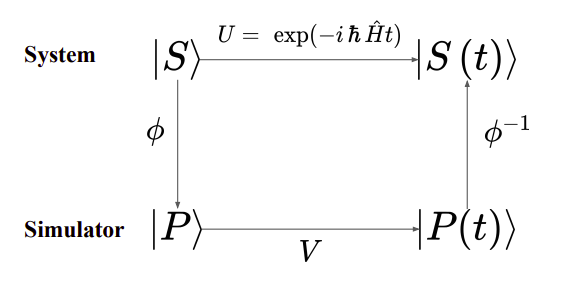
\includegraphics[width=\textwidth]{fig_10.png}}
	\centering
	\caption{$\ket{S}$ and $\ket{S(t)}$ represent the initial and final state (time evolved state) of system. Similarly, $\ket{P}$ and $\ket{P(t)}$ represent initial and final state of the simulator. }
	\label{fig 10}
\end{figure}
Here the system is mapped to the simulator via an invertible map $\phi$ ( operator ). This mapping determines the correspondence between the states and operators of the system and simulator.\par
If we follow such a scheme described by figure $\ref*{fig 10}$, the evolution operator $U$ and $ V$ would be connected by,
\begin{equation}
V = \phi U \phi^{-1}
\end{equation}
If mapping is unitary, we can write,
\begin{equation}
V = e^{- i \hbar H_{sim} t}
\end{equation}
Where $H_{sim} = \phi H_{sys} \phi^{-1}$.\par
Thus while simulation we map the initial state $\ket{S}$ to $\ket{P}$
\begin{equation}
\ket{P} = \phi \ket{S} 
\end{equation}
Then simulator is allowed to time evolve $\ket{P} \xrightarrow{V} \ket{S}$. After time evolution final state $\ket{P(t)}$ is mapped back to $\ket{S(t)}$.
\begin{equation}
\ket{P(t)} = \phi^{-1}\ket{S(t)}
\end{equation}
Thus eventually we get back the time evolution of the system $\ket{S} \rightarrow \ket{S(t)}$.

Now we are going to discuss a very simple scheme of mapping between quantum system and simulator. The scheme we are discussing is proposed by Somaroo et al. (1999)\cite{somaroo} for simulating a quantum harmonic oscillator on two proton nuclear spins in 2,3-dibromothiophene. Note that here the number of states available for QHO is restricted to $4$. The convenient unitary mapping of system and simulator is,
\begin{gather*}
\ket{n=0} \leftrightarrow \ket{\uparrow\uparrow}
\ket{n=1} \leftrightarrow \ket{\uparrow\downarrow}
\ket{n=2} \leftrightarrow \ket{\downarrow\uparrow}
\ket{n=3} \leftrightarrow \ket{\downarrow\downarrow}
\end{gather*}
One doesn’t need to have followed this mapping. The mapping presented above is simple and straight forward. \par
The time evolution operator of QHO is given by
\begin{equation}
U = e^{-i\hbar H_{QHO} t} \equiv \exp\left[-i\left(\frac{1}{2}\ket{0}\bra{0} + \frac{3}{2}\ket{1}\bra{1} + \frac{5}{2}\ket{2}\bra{2} + \frac{7}{2}\ket{3}\bra{3}\right)\hbar\omega t\right]
\end{equation}
Where $\omega$ is the oscillatory frequency. From this, we can find the time evolution of the simulator.
\begin{equation}
\label{eq:19}
V = e^{-i\hbar H_{sim} t} \equiv \exp\left[-i\left(\frac{1}{2}\ket{\uparrow\uparrow}\bra{\uparrow\uparrow} + \frac{3}{2}\ket{\uparrow\downarrow}\bra{\uparrow\downarrow} + \frac{5}{2}\ket{\downarrow\uparrow}\bra{\downarrow\uparrow} + \frac{7}{2}\ket{\downarrow\downarrow}\bra{\downarrow\downarrow}\right)\hbar\omega t\right]
\end{equation}
In Pauli basis ${\sigma_{x},\sigma_{y},\sigma_{z},I}$, equation $\ref{eq:19}$ can be rewritten as ,
\begin{equation}
\label{eq:20}
V = exp\left[i\left(\sigma_{z}^{2}(1 + \frac{1}{2}\sigma_{z}^{2}) - 2 \right)\omega t\right]
\end{equation} 
Thus the simulator evolves according to equation $\ref{eq:20}$. At the end of the simulation, final state of the simulator is measured. The resultant state is mapped back into the QHO state.\par

Sometimes we can simulate not able to simulate the entire system. But mapping can be done in such a way that it could be used to study some characteristic of the system. In general, the mapping we use depends upon the characteristic of the system we intend to study and the properties of the simulator. In AQS the physical quantities can be measured directly from the simulator. Since it is analogous to the system, measurement results yield information about the system. This is an added advantage since in DQS we need to computationally manipulate the measurement results. Also in AQS even if there are we can use it to perform qualitative studies. But the error rate should be below a tolerance level. In such cases, AQS can be used to investigate properties like phase transition.  

Now in the example, we have shown, the mapping was simple and straight forward. But generally, this is not the case. Sometimes clever mapping schemes have to formulated to efficiently simulate a system. Further discussion in this direction can be seen in the reference \cite{georgescu}.

\newpage
\thispagestyle{empty}
\mbox{}
\newpage
\chapter{Neutrino Oscillation}
\section{Introduction}
A neutrino  ( represented by the Greek letter $\nu$) is a fermion an elementary particle with a spin of $\frac{1}{2}$ undergo interaction only via the weak interaction and gravity. Pauli proposed neutrino to be a non-interacting, neutral particle to recover conservation laws in the case of beta decay which was then appeared to violate it. Even though they are abundant in-universe since they undergo only weak interaction, they rarely interact with matter and thus are incredibly difficult to detect. The first detection of neutrino only occurred 25 years after it was first proposed. Two American physicists Clyde Cowan and Frederick Reines detected anti neutrinos which were emitted by a nuclear reactor and were awarded Nobel Prize for their discovery.\par
During weak interactions neutrinos are created in one of the three leptonic flavours: electron neutrinos ($\nu_{e}$), muon neutrinos ($\nu_{\mu}$), or tau neutrinos ($\nu_{\tau}$), in association with the corresponding charged lepton. The three neutrino flavours appear to be distinct: For instance, when muon-neutrinos interact with a target, they will always produce muons, and never taus or electrons. Although they were long believed to be massless, it is now known that there are three discrete neutrino masses with different tiny values, but they do not correspond uniquely to the three flavours. A neutrino created with a specific flavour has an associated specific quantum superposition of all three mass states. As a result, neutrinos oscillate between different flavours in flight. For example, an electron neutrino produced in a beta decay reaction may interact in a distant detector as a muon or tau neutrino. Neutrino oscillation arises from the mixing between the flavour and mass eigenstates of neutrinos. That is, the three neutrino states that interact with the charged leptons ($\nu_{e}$, $\nu_{\mu}$ or $\nu_{\tau}$) in weak interactions are each a different superposition of the three (propagating) neutrino states of definite mass (Let say $\nu_{1},\nu_{2},\nu_{3}$). Neutrinos are emitted and absorbed in weak interaction processes in flavour eigenstates but travel as mass eigenstates\cite{Aartsen}. Mass eigenstates have definite masses and since they are slightly different from each other as they propagate each of them advance at slightly different rates. This results in a changing superposition mixture of mass eigenstates as the neutrino travels, but a different mixture of mass eigenstates corresponds to a different mixture of flavour states. So a neutrino born as, say, an electron neutrino will be some mixture of an electron, muon, and tau neutrino after travelling some distance. Since the quantum mechanical phase advances in a periodic fashion, after some distance, the state will nearly return to the original mixture, and the neutrino will be again mostly electron neutrino. The electron flavour content of the neutrino will then continue to oscillate – as long as the quantum mechanical state maintains coherence. Since mass differences between neutrino flavours are small in comparison with long coherence lengths for neutrino oscillations, this microscopic quantum effect becomes observable over macroscopic distances.\par
A practical method for investigating neutrino oscillations was first suggested by Bruno Pontecorvo in 1957 using an analogy with kaon oscillations; over the subsequent 10 years, he developed the mathematical formalism and the modern formulation of vacuum oscillations. In 1985 Stanislav Mikheyev and Alexei Smirnov (expanding on 1978 work by Lincoln Wolfenstein) noted that flavour oscillations can be modified when neutrinos propagate through matter. This so-called Mikheyev Smirnov Wolfenstein effect (MSW effect) is important to understand because many neutrinos emitted by fusion in the Sun pass through the dense matter in the solar core (where essentially all solar fusion takes place) on their way to detectors on Earth. This phenomenon which revealed through experiments that helped in solving the long-standing solar neutrino problem. Additionally, this observation that neutrino change from one flavour shed light on several characteristics of neutrino, in particular, indicated that neutrinos have non zero masses, which requires the modification of the standard model of particle physics. This experimental discovery of neutrino oscillation and thereby non zero mass by Super Kamiokande and Sudbury neutrino observatory won the Nobel prize for physics in 2015.

\section{Neutrino Flavour Oscillation in Vaccum}
A typical Neutrino flavour change is depicted in the figure $\ref*{fig 1}$. A neutrino source produces a neutrino along with charged lepton.Flavour of the lepton ($e,\mu$,or $\tau$) produced would give us the flavour of neutrino produced ($\nu_{e},\nu_{\mu}$,or $\nu_{\tau}$). A neutrino created in a specific flavour eigenstate would be in coherent superposition of all three mass eigenstates. This is coherent superposition impies that we cannot experimentally find out which mass state is produced at the interaction vertex of feynman diagram. But the proportion of each mass state in the produced pure flavour state has been found to depend profoundly on that flavour. The relationship between flavour and mass states is encoded in the PMNS (Pontecorvo Maki Nakagawa Sakata) matrix. It is a unitary mixing matrix that contains information on the mismatch of quantum states of neutrinos when they propagate freely and when they take part in the weak interactions. Experiments have established values for the elements of this matrix\cite{zyla}.\par
\begin{figure}[h]
\graphicspath{ {./Images/} }	
{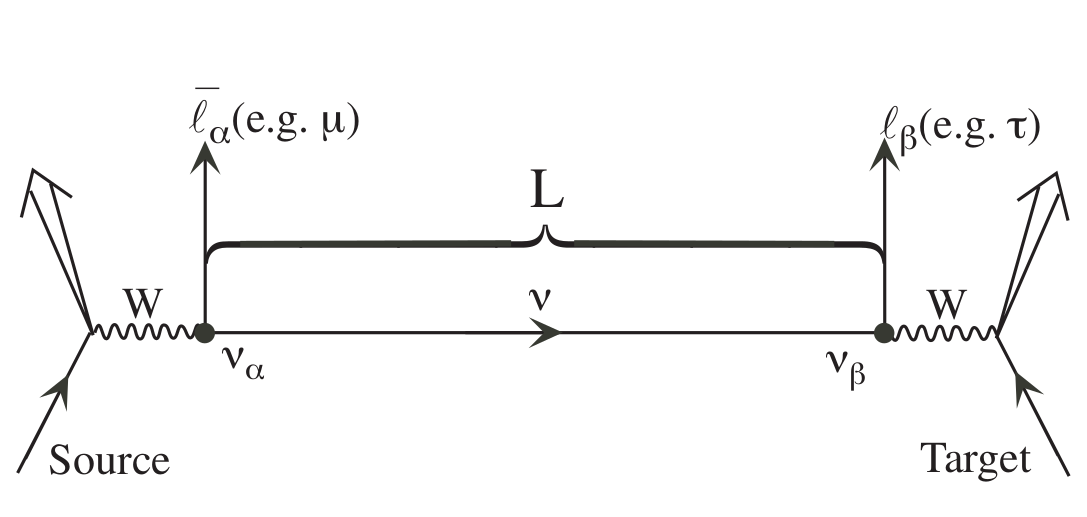
\includegraphics[width=\textwidth]{fig_1.png}}
\centering

\caption{ Neutrino flavour change in vaccum\cite{kayser}.}
\label{fig 1}
\end{figure}


Experimentally a neutrino beam of known flux and flavour $\alpha$ is produced and send to a detector placed at a distance $L$ from the source. There it would interact with the detector material to produce a secondary lepton, let say $l_{\beta}$.  Thus at the time of interaction(with detector material), the neutrino would in $\beta$ flavour state ( $\nu_{\beta}$ ). One could detect the flavour change in two ways. One way is observe the appearance of neutrinos of new flavour $\beta$ that is different from the original flavour ( $\beta\neq\alpha$). Such type of experiments are called appearance experiments and would give appearance probability. The other way to is to observe thatsome of this known flavour $\nu_{\alpha}$ disappears. Such type of experiments are called disappearance experiments and would give disappearance probability or survival probability.

\subsubsection{Theory of Flavour Oscillation}
In order to explain the phenomenon of oscillations, one has to decompose a flavour eigenstate $\ket{\nu_{\alpha}}$ in the mass eigenstate basis $\ket{\nu_{i}}$. In a simple sense mass eigenstates are the eigenstates of the hamiltonian. Flavour states (for eg: $\nu_{\mu}$, $\nu_{e} $ ) are not eigenstates of the hamiltonian and thus do not have definite energy eigenvalue. A mass eigenstate of type $i$ with momentum $p_{i}$ is an energy eigenstate with eigenvalues  $E_{i}=\sqrt{p_i^{2}+m_{i}^{2}}$ . Flavour and mass eigenstates are connected via PMNS Matrix which is unitary. The matrix equation connecting flavour and mass states are given by:
\begin{gather}
 \begin{bmatrix} \ket{\nu_{e}} \\ \ket{\nu_{\mu}} \\ \ket{\nu_{\tau}} \end{bmatrix} = 
 \begin{bmatrix} U_{e1} & U_{e2} & U_{e3} \\ U_{\mu 1} & U_{\mu 2} & U_{\mu 3}\\ U_{\tau 1} & U_{\tau 2} & U_{\tau 3}\end{bmatrix} \begin{bmatrix} \ket{\nu_{1}} \\ \ket{\nu_{2}} \\ \ket{\nu_{3}} \end{bmatrix}
\end{gather}
Thus a flavour state $\alpha$ can be written as a superposition of mass eigenstate.
\begin{equation}
\label{eq:0a}
	\ket{\nu_{\alpha}}=\sum_{i = 1,2,3} U^{\dagger} _{\alpha i}\ket{\nu_{i}}
\end{equation}
Where $\alpha = e,\mu,\tau$  and quantities  may be collected into a matrix known as PMNS matrix or Leptonic mixing matrix. According to Standard Model $U$ must be unitary. This guarantees that when a neutrino $\nu_{\alpha}$ interacts in a detector it would produce a lepton of the same flavour. The relation connecting a particular flavour state to mass eigenstate can be inverted to express a mass eigenstate in terms of flavour state.
\begin{equation}
\label{eq:0b}
\ket{\nu_{i}}=\sum_{\alpha = e,\mu,\tau} U_{\alpha i}\ket{\nu_{\alpha}}
\end{equation}
Where $|U_{\alpha i}|^{2}$ the probability that $\nu_{i}$ interacts with a detector to produce a charged lepton of the flavour of $\alpha$. When standard three flavour oscillation is considered the PMNS matrix is 3x3 in nature and for two flavour oscillation, it is 2x2. It is given by
\begin{equation}
\label{eq:0c}
U = \begin{bmatrix} C_{12}C_{13} & S_{12}C_{13} & S_{13}e^{i\delta} \\
S_{12}C_{23}-C_{12}C_{23}S_{13}e^{i\delta} & S_{12}C_{23}-S_{12}S_{23}S_{13}e^{i\delta}& S_{23}C_{13}\\
S_{12}S_{23}-C_{12}C_{23}S_{13}e^{i\delta}& -C_{12}S_{23}-S_{12}C_{23}S_{13}e^{i\delta}&C_{23}C_{13} \end{bmatrix} \begin{bmatrix}
e^{\frac{i\alpha_{1}}{2}}&0&0\\0& e^{\frac{i\alpha_{2}}{2}}&0\\0&0&0\end{bmatrix}
\end{equation}
Where $C_{ij}=cos(\theta_{ij})$, $S_{ij}=sin(\theta_{ij})$. The phase factors $\alpha_{1}$ and $\alpha_{2}$ (Majarona phases) are physically meaningful only if neutrinos are Majorana particles ( i.e. if the neutrino is identical to its antineutrino) and do not enter into oscillation phenomena regardless. The phase factor $\delta$ known as the Dirac phase is non-zero only if neutrino oscillation violates CP symmetry, this has not yet have been experimentally observed. So in our discussion for convenience, we take $\delta$ and $\alpha_{i}$ to be zero. In the presence of an additional neutrino, which is called a sterile neutrino and not yet have been experimentally observed, the PMNS matrix gets modified into a 4x4 matrix.\par

For simplicity, we first discuss two flavour neutrino oscillation even though all 3 neutrinos take part in neutrino oscillation. But two neutrino oscillation is a fairly accurate description of a number of experiments. For example, $\nu_{\mu} \rightarrow \nu_{\tau}$ transitions are relevant for atmospheric neutrinos,$\nu_{e}\rightarrow \nu_{\alpha}$ in solar neutrinos, $\nu_{e}\rightarrow\nu_{\mu}$  at reactor experiments and $\nu_{\mu} \rightarrow \nu_{e}$ at accelerator experiments \cite{Blasome}.\par

Suppose we generate a neutrino beam containing a flavour state $\alpha$ which describes the flavour of neutrino at $(x,t)$. Now, if we send the neutrino beam along the x-axis and let them propagate in a free space towards a detector some distance L. Then mass eigenstates propagate according to the time-dependent Schrodinger equation with no potentials.
\begin{equation}
i\frac{d\ket{\nu_{i}(x,t)}}{dx}=E_{i}\ket{\nu_{i}(x,t)}
\end{equation}
Here quantities are expressed in natural units (c = $\frac{h}{2\pi}$ = 1) and $E_{i}$ is the energy corresponding to the mass eigenstate $\nu_{i}$.\par
The solution of this equation is a plane-wave : 
\begin{equation}
\label{eq:0}
\ket{\nu_{i} (x,t)} = e^{-i\phi_{i}}\ket{\nu_{i} (0,0)}
\end{equation}
Where $\phi_{i}$ is the phase factor picked up by neutrino during propagation.\par
At some later space-time point (x,t) the flavour state $\alpha$ will be : 
\begin{equation}
\label{eq:1}
\ket{\nu_{\alpha}(x,t)} = \sum_{i=1,2} U_{\alpha i}^{\dagger} e^{-i\phi_{i}}\ket{\nu_{i}(0,0)}
\end{equation}
Inverting the mixing matrix we can write ;
\begin{equation}
\label{eq:2}
\ket{\nu_{i}(0,0)} = \sum_{\gamma} U_{\gamma i} \ket{\nu_{\gamma}(0,0)}
\end{equation}
Substituting $\ref{eq:2}$ in $\ref{eq:1}$ , we can write the flavour state as 
\begin{gather*}
\ket{\nu_{\alpha} (x,t)} =  \sum_{i=1,2} U_{\alpha i}^{\dagger}e^{-i\phi_{i}}\ket{\nu_{i}(0,0)}
\sum_{\gamma} U_{\gamma i} \ket{\nu_{\gamma}(0,0)}\\
 = \sum_{i}\sum_{\gamma} U_{\alpha i}^{\dagger} e^{-i\phi_{i}} U_{\gamma i} \ket{\nu_{\gamma}(0,0)}
\end{gather*}
Thus the amplitude of a detecting a neutrino flavour $\beta$ at a position $(x,t)$ given that we generate a neutrino flavour $\alpha$ at a position $(0,0)$.
\begin{equation}
\begin{split}
A(\nu_{\alpha} (0,0)\rightarrow\nu_{\beta}(0.0))& = \braket{\nu_{\beta}(x,t)|\nu_{\alpha}(0,0)}\\
& =\sum_{\gamma}\sum_{i} U_{\gamma i}e^{i\phi_{i}}U_{\beta i}^{\dagger}\braket{\nu_{\gamma}(0,0)}{\nu_{\alpha}(0,0)}\\
& =\sum_{k}U_{\alpha i}^{\dagger}e^{i\phi_{i}}U_{\beta i}
\end{split}
\end{equation}
Where last step comes from the orthogonality of flavour state $\braket{\nu\gamma(0,0)|\nu\alpha(0,0)} =\delta_{\gamma\alpha}$. 
The oscillation probability is given by :
\begin{equation}
\label{eq:3}
\begin{split}
P(\nu_{\beta} \rightarrow\nu_{\alpha})& =|A(\nu_{\beta}(0,0)\rightarrow\nu_{\alpha}(x,t))|^{2}\\
&=|\sum_{i}U_{\alpha i}^{\dagger} e^{i\phi_{i}}U_{\beta i}|^{2}\\
&=\sum_{i}\sum_{j}U_{\alpha i} U_{\beta i}^{\dagger} U_{\alpha j }^{\dagger}U_{\beta j}e^{-i(\phi_{j}-\phi_{i})}
\end{split}
\end{equation}

For two flavour oscillation, $U$ would be a 2x2 rotation matrix. The rotation matrix would rotate a vector in the flavour basis into a vector in the mass basis

\begin{equation}
U= \begin{bmatrix}cos(\theta) & -sin(\theta) \\ sin(\theta) & cos(\theta) \end{bmatrix}	
\end{equation}
So that,
\begin{equation}
\begin{bmatrix} \nu_{\alpha} \\ \nu_{\beta} \end{bmatrix} = \begin{bmatrix} cos(\theta) & \sin(\theta) \\ -sin(\theta) & cos(\theta) \end{bmatrix}\begin{bmatrix} \nu_{i} \\ \nu_{j} 
\end{bmatrix}
\end{equation}
Where $\theta$ is called mixing angle. This will have to be measured in the experiment. 
Using the form of $U$ we can work out a relation for oscillation probability by substituting it in the \ref{eq:3}. On reduction, we could arrive at an equation of oscillation probability in terms of mixing angle and $\phi$ as:
\begin{equation}
\label{eq:3a}
P(\nu_{\alpha} \rightarrow \nu_{\beta}) = sin^{2}(2\theta)sin^{2}(\frac{\phi_{i}-\phi_{j}}{2})
\end{equation}

In lab frame, since assumed to be plane waves $\phi_{i}$ can be written as ;
\begin{equation}
\phi_{i} = E_{i} t - p_{i}x
\end{equation}

To proceed further, we make a shady approximation. Usually, we assume the mass eigenstates either created with the same momentum or with the same energy. Since neutrino flavour is measured by observing charged leptons which is Lorentz invariant, the oscillation probability must be Lorentz invariant. But the relativistic transformation of energy and momentum implies that the equal momentum assumption cannot hold in different inertial frames\cite{giunti2003}. Thus one has to assume all $E_{i}$’s as equal\cite{stodolsky}\cite{lipkin}\cite{obkun}. Otherway to put it is that only components in the neutrino beam having the same energy contribute coherently to a neutrino oscillation signal.  The fact we need to make such an approximation come from our modelling of neutrino mass eigenstates as plane waves. If we model neutrino mass eigenstates as wave packets, we need not make any approximation and get the same results. But the mathematical treatment of such a model is never so easy mathematically \cite{giunti1991}\cite{giunti1998}\cite{giunti2004}. Nevertheless, it has been found out that wave packet description is unnecessary while dealing with stationary sources. For stationary systems, all information necessary for single-particle measurements is contained in the energy spectrum; and the sun or the reactor or even a supernova for most purposes can certain only be regarded as essentially stationary sources\cite{stodolsky}. \par
At energy $E_{i}$, mass eigenstate $\nu_{i}$ of mass $m_{i}$ have momentumin the ultra relativistic limit.
\begin{equation}
\label{eq:4}
p_{i} = \sqrt{ E^{2} - m_{i}^{2}} \cong E-\frac{m_{i}^{2}}{2E}
\end{equation}
The expression $E = m^{2}c^{4} + p^{2}c^{2}$ gives the relativistic energy of a particle with rest mass m and momentum p. In the ultra-relativistic limit, energy would be almost completely contributed by the momentum part ( $ p^{2}c^{2} \gg mc^{2}$ ) and thus can be approximated by $ E \approx pc $. In equation $\ref{eq:4}$ we have used the fact that $m_{i}^2 \ll E^{2}$ in ultra-relativistic limit. Thus,
\begin{equation}
\label{eq:5}
\phi_{i} \cong E( t - L) + \frac{m_{i}^2 L}{2E}
\end{equation}
Where L is the distance of separation between the source and the detector.\par
In the equation, $\ref{eq:5}$  the term $ E( t - L)$ act as a global phase (same for all mass eigenstates) and hence can be treated as irrelevant as no interesting physics happens with it. Thus equation $\ref{eq:5}$ becomes :
\begin{equation}
\label{eq:6}
\phi_{i} = \frac{m_{i}^2 L}{2E}
\end{equation}
Substituting $\ref{eq:6}$  in  $\ref{eq:0}$  we would get that,
\begin{equation}
\ket{\nu_{i} (L,t)} = e^{\frac{-i m_{i}^2 L}{2E}}\ket{\nu_{i} (0,0)}
\end{equation}
As propagating, the mass eigenstates gain a quantum mechanical phase which depends upon the$ m_{i}$ and $L$ ( For constant $E$ ). Since the mass eigenstates are combinations of flavour eigenstates, interfere with the corresponding flavour components of each mass eigenstate. Constructive interference causes it to be possible to observe a neutrino created with a given flavour to change its flavour during its propagation. The probability of a neutrino oscillates to another flavour ( termed as ‘Appearance probability’ ) is given by the equation $\ref{eq:3a}$. Then 
\begin{equation}
\label{eq:6a}
\phi_{j} - \phi_{i} = \frac{m_{j}^{2}}{2E} - \frac{m_{i}^2}{2E} = \frac{\Delta m^{2} L}{2E}
\end{equation} 
Where $\Delta m^{2} = m_{j}^{2}-m_{i}^{2}$.
Substituting back into $\ref{eq:3a}$ we get 
\begin{equation}
\label{eq:7}
P(\nu_{\alpha} \rightarrow \nu_{\beta}) = sin^{2}(2\theta)sin^{2}( \frac{\Delta m^{2} L}{4E})
\end{equation}
If we agree to measure L in units of kilometres and E in GeV and put back $\hslash$ and $c$ which was earliwer left out into $\ref{eq:7}$,
\begin{equation}
\label{eq:8}
P(\nu_{\alpha} \rightarrow \nu_{\beta}) = sin^{2}(2\theta)sin^{2}( \frac{1.27\Delta m^{2} L}{E})
\end{equation}
The corresponding survival probability ( or disappearance probability) that is generating an $\alpha$ flavour neutrino and detecting the same flavoured neutrino is given by,
\begin{equation}
\label{eq:9}
P(\nu_{\alpha} \rightarrow \nu_{\alpha}) = 1-sin^{2}(2\theta) sin^{2}( \frac{1.27\Delta m^{2} L}{E})
\end{equation}
The same mathematical treatment an can be used in the case of three flavour to develop theory of Three flavour oscillation. Using the equation $\ref{eq:0a}$, we can write $\nu_{\alpha}$ at $x=0$, $t=0$ as;
\begin{equation}
\ket{\nu_{\alpha}(0,0)}= U_{\alpha 1}^{\dagger}\ket{\nu_{1}}+U_{\alpha 2}{\dagger}\ket{\nu_{2}})+ U_{\alpha 3}^{\dagger}\ket{\nu_{3}}
\end{equation}
After travelling a distance of L the state of the state of neutrino would be ( given by $\ref{eq:0}$ );
\begin{equation}
	\label{eq:10}
	\ket{\nu_{\alpha}(x,t)} = U_{\alpha 1}^{\dagger} e^{i\phi_{1}}\ket{\nu_{1}}+U_{\alpha 2}^{\dagger}e^{i\phi_{2}}\ket{\nu_{2}})+ U_{\alpha 3}^{\dagger}e^{i\phi_{3}}\ket{\nu_{3}}
\end{equation}

Where $\phi_{i} = E_{i}t - p_{i}x$ .For a detector placed at distance L from the source, in the ultra-relativistic limit, $\phi_{i} \cong \frac{m_{i}^{2}L}{2E_{i}} $. Thus state evolution can be expressed in terms of L alone. \par
Expressing the mass eigenstates in terms of the flavour eigenstates ( refer $\ref{eq:0b}$ ) in equation $\ref{eq:10}$,
\begin{equation}
\begin{split}
\ket{\nu_{\alpha}(L)}&=(U_{\alpha 1}^{\dagger}U_{e1}e^{-i\phi_{1}}+U_{\alpha 2}^{\dagger}U_{e2}e^{-i\phi_{2}}+U_{\alpha 1}^{\dagger}U_{e3}e^{-i\phi_{3}})\ket{\nu_{e}}\\
&+(U_{\alpha 1}^{\dagger}U_{\mu 1}e^{-i\phi_{1}}+U_{\alpha 2}^{\dagger}U_{\mu 2}e^{-i\phi_{2}}+U_{\alpha 1}^{\dagger}U_{\mu 3}e^{-i\phi_{3}})\ket{\nu_{\mu}}\\
&+(U_{\alpha 1}^{\dagger}U_{\tau 1}e^{-i\phi_{1}}+U_{\alpha 2}^{\dagger}U_{\tau 2}e^{-i\phi_{2}}+U_{\alpha 1}^{\dagger}U_{\tau 3}e^{-i\phi_{3}})\ket{\nu_{\tau}}
\end{split}
\end{equation}
Thus oscillation probability $P(\nu_{\alpha} \rightarrow \nu_{\beta})$ is given by,
\begin{equation}
\label{eq:11}
\begin{split}
P(\nu_{\alpha} \rightarrow \nu_{\beta})& = |\braket{\nu_{\beta}|\nu_{\alpha}}|^{2}\\
&=(U_{\alpha 1}^{\dagger}U_{\beta 1}e^{-i\phi_{1}}+U_{\alpha 2}^{\dagger}U_{\beta 2}e^{-i\phi_{2}}+U_{\alpha 1}^{\dagger}U_{\beta 3}e^{-i\phi_{3}})
\end{split}
\end{equation}
On solving equation $\ref{eq:11}$ we could derive a form for $P(\nu_{\alpha} \rightarrow \nu_{\beta})$ as
\begin{equation}
\label{eq:12}
P(\nu_{\alpha} \rightarrow \nu_{\beta}) = \delta_{\alpha\beta} - 4\sum_{i>j}(U_{\alpha i}U_{\beta i}U_{\alpha j}U_{\beta j}) sin^{2}(\Delta m_{ij}^{2} \frac{L}{4E})
\end{equation} 
While solving equation $\ref{eq:11}$  we assume that the Dirac phase, $\delta = 0$ that is there is no charge parity violation. \par
Let us consider an appearance experiment ( $\alpha \neq \beta$ ). Then, 
\begin{equation}
\label{eq:13}
\begin{split}
P(\nu_{\alpha} \rightarrow \nu_{\beta} )& = -4\sum_{i>j} ( U_{\alpha i} U_{\beta i} U_{\alpha j} U_{\beta j}) sin^{2}( \frac{1.27 \Delta m_{ij}^{2}  L}{E})\\
&=-4[ ( U_{\alpha 1} U_{\beta 1} U_{\alpha 2} U_{\beta 2})sin^{2}( \frac{1.27\Delta m_{12}^{2} L}{E})\\
&+( U_{\alpha 1} U_{\beta 1} U_{\alpha 3} U_{\beta 3})sin^{2}( \frac{1.27\Delta m_{13}^{2} L}{E})\\
&+( U_{\alpha 2} U_{\beta 2} U_{\alpha 3} U_{\beta 3})sin^{2}( \frac{1.27\Delta m_{23}^{2} L}{E})]
\end{split}
\end{equation}
Since there are 3 mass states there would be 2 independent mass splittings, called $\Delta m_{23}^{2}$ and $\Delta m_{12}^{2}$. The other splitting is defined by the relation $\Delta m_{12}^{2}$+$\Delta m_{23}^{2}$+$\Delta m_{13}^{2}$ = 0. From solar and atmospheric neutrino problems it is measured that $\Delta m_{12}^{2}\sim 10^{-5}$ and $\Delta m_{23}^{2} \sim 10^{-3}$. Thus at reasonable approximation $\Delta m_{23}^{2} \approx \Delta m_{13}^{2}$ at low $\frac{L}{E}$ limit we can approximate $\ref{eq:13}$ as
\begin{equation}
\label{eq:14}
P(\nu_{\alpha} \rightarrow \nu_{\beta} ) =-4 [ U_{\alpha 1} U_{\beta 1} U_{\alpha 3} U_{\beta 3} + U_{\alpha 2} U_{\beta 2} U_{\alpha 3} U_{\beta 3}]sin^{2}( \frac{1.27\Delta m_{23}^{2} L}{E})
\end{equation}
Through experiments we can determine the mixing angle ($ \theta_{ij}$) and mass splitings ($\Delta m_{ij}$). By substituting it into the matrix given by $\ref{eq:0c}$ we can find out PMNS matrix (assume $\delta$,$\alpha$ = 0). Substituting the matrix elements back into $\ref{eq:14}$ would give probability neutrino of a particular flavour to oscillate at a distance $L$ from the source.
\newpage
\thispagestyle{empty}
\mbox{}
\newpage
\chapter{Neutrino Oscillation in a quantum processor}
\section{Introduction}
The spontaneous transition of neutrino flavour over a macroscopic distance occurs due to the non-coinciding of flavour and mass eigenstates called Neutrino Oscillation.  Neutrino oscillation through its periodic nature has given insights that neutrinos have non zero mass, which is something beyond the Standard Model’s predictions. Thus neutrino oscillations indicate the existence of physics outside the standard model. Experimentally when we study neutrino oscillation what we do inspect the neutrino oscillation behaviour at different values of energies E and baseline L. For different $L/E$ values, we perform either appearance experiment (or disappearance experiment) and get appearance probability ( or disappearance probability). Using experimentally obtained probabilities we would fix the values of the mixing angle ($\theta_{ij}$) and squared mass difference ( $\Delta m_{ij}^{2}$) by putting them back into the corresponding equation. \par
Often detectors depending upon the type, work at different energy range and threshold energy below which detection of neutrinos is not possible. For example, detectors using water as detector material, detect neutrinos via elastic scattering will not work for neutrinos of low energy ( $< 5 MeV$). Similarly, Chlorine-based detectors have a threshold of 0.814 MeV.\par
Another thing that often concerns the experimentalist is the sensitivity of the detectors. In the case of reactor-based or accelerator-based experiments sensitivity of the detector depends upon the baseline length. For eg, for a neutrino beam of energy $E \sim 1 GeV$ detector baseline should be at least of the order of $10^{4}$  for it to be sensitive to $\Delta m_{ij}^{2}$ down to $\sim 10^{-4} eV^{2}$. Using the experimentally got parameters, we can perform simulational studies of the flavour oscillation for neutrino beams of energies inaccessible under lab conditions.\par
Not so long after Feynman put forward the idea of simulating a quantum system with another, the possibility of using a quantum computer to simulate quantum systems was understood. The major difference between a classical computer and a quantum computer in simulating quantum systems is that the quantum computer performs actual Hamiltonian evolution whereas others just emulate it. At the present stage, even though the result got by quantum simulations is not praiseworthy as that of classical simulations, the computational cost of quantum algorithms are much less compared to classical algorithms for simulating a quantum system. The development of fault torrent quantum computation would give us more reliable results enable us to manoeuver the quantum advantage in a wide variety of fields.\par
Here we perform quantum simulation by executing an analogous Hamiltonian evolution to generate neutrino flavour oscillation. Such encoding and evolution is a vital building block on which more advanced quantum simulations involving neutrino flavour can be constructed. Systems that could particularly benefit from the quantum algorithmic approach to neutrino flavour evolution include those where collective neutrino oscillations are relevant, such as in Supernovae or the early Universe \cite{jones}. In such cases, the quantum Boltzmann equation which gives the evolution neutrino population can only be solved approximately. \par
In this section, we are going to first discuss how to encode two neutrino system evolution on a quantum computer using only a single qubit. Now, then we extend this idea to implement three flavour oscillation in a 2 qubit space inside a quantum processor. While simulating, the primary challenge that lies ahead is to implement the PMNS matrix which relates the flavour and mass eigenstates. Here we use the algorithm or the circuit put forward by Arg\"uelles et.al 2019, to study neutrino flavour oscillation. This algorithm uses quantum gates to realise the PMNS matrix and to realise the time evolution operator. The algorithm is discussed below.
\section{Simulation of two flavour oscillation}\label{2FO}
In this circuit we only use a single qubit to encode neutrino flavour state and to time evolve the states we apply corresponding quantum gates. Let our system have of two neutrino flavour state let say $\alpha$ and $\beta$. Now we want to encode these states on qubits and encoding scheme we follow is given below.
\begin{equation}
\begin{split} 
\label{eq:14}
\ket{\nu_{\alpha}}=\begin{bmatrix} 1 \\ 0 \end{bmatrix} , 
\ket{\nu_{\beta}}=\begin{bmatrix} 0 \\ 1 \end{bmatrix}
\end{split}
\end{equation}
In the case of two flavour oscillation is the PMNS matrix is given by the 2x2 rotation matrix.
\begin{equation}
U=\begin{bmatrix} cos(\theta) & \sin(\theta) \\ -sin(\theta) & 
cos(\theta) \end{bmatrix}
\end{equation}
PMNS operation is encoded in  IBM Quantum computer by three-parameter U gate. The matrix form of the gate is given as :
\begin{equation}
	\label{eq:15}
	U (\Theta,\Phi,\Lambda) =\begin{bmatrix} cos(\frac{\Theta}{2}) & -\sin(\frac{\Theta}{2})e^{i\Lambda} \\ sin(\frac{\Theta}{2})e^{i\Phi} & 
		cos(\frac{\Theta}{2})e^{i(\Lambda + \Phi)} \end{bmatrix}
\end{equation}

For a two-neutrino system, the oscillation probabilities depend upon a single parameter known as mixing angle. Thus the U gate which having 3 parameters has to be modified,
\begin{enumerate}
	\item Now consider the case of including the parameter $\Phi$. This corresponds to the rephasing of charged lepton field, and standard Lagrangian is invariant under such an operation. For eg, let us consider the case of a muon neutrino. The presence of $\Phi$ corresponds to rephasing $\ket{\nu_{\mu}}$ by $e^{-i\Phi}\ket{\nu_{\mu}}$. As said before, under such a transformation Lagrangian remains invariant and does not influence oscillation probabilities \cite{giunti2007}. Thus we can take $\Phi = 0$ without loss of any generality.
	\item We can use the same arguments provided above to set $\Lambda = 0$ for the case of Dirac fermions\cite{giunti2007}. But this is not possible in the case of neutrino being a Majorana particle. For Majorana particle, this phase is physical and should be maintained in the Langrangian. However, it is proven the presence of such a phase would not affect the oscillation probabilities\cite{giunti2010} and thus can be taken equal to zero while studying the neutrino oscillation irrespective of the type of particle.
\end{enumerate}
Thus using a U gate we can realise the PMNS matrix by suitably choosing the value of the parameters. 
\begin{equation}
\label{eq:16}
U_{PMNS}^{2x2} = U(-2\theta,0,0) = \begin{bmatrix} cos(\theta) & \sin(\theta) \\ -sin(\theta) & 
cos(\theta) \end{bmatrix}
\end{equation}
Where $\theta$ is the mixing angle.\par

Using the PMNS matrix that we realised using U gate, flavour state encoded in the qubit $\ref{eq:14}$ can be rotatated into in the mass basis ($\ket{\nu_{1}},\ket{\nu_{2}}$). After rotating into mass basis we have to time evolve the mass states. From $\ref{eq:1}$ we know that,
\begin{gather*}
\begin{split}
\ket{\nu_{\alpha}(t)}& = U_{\alpha 1}^{\dagger}e^{i\phi_{1}}\ket{\nu_{1}} + U_{\alpha 2}^{\dagger}e^{i\phi_{2}}\ket{\nu_{2}}\\
&=e^{i\phi_{1}}( U_{\alpha 1}^{\dagger}\ket{\nu_{1}} + U_{\alpha 2}^{\dagger} e^{ i\Delta\phi}\ket{\nu_{2}}
\end{split}
\end{gather*}
Where $\Delta\phi=\phi = \phi_{2}-\phi_{1}$.
Global phases like $e^{i\phi_{1}}$ have no physical significance and can be discarded\cite{benenti}, relative phases between mass states are only relevant for neutrino oscillations, and without losing any generality we can measure all phases relative to $\ket{\nu_{1}}$ state. Thus time evolution operator can also be encoded by using a U gate.
\begin{equation}
U(t) = U(0,0,\phi) = \begin{bmatrix} 1 & 0 \\ 0 & e^{i\phi} \end{bmatrix}
\end{equation}
Where $\phi = \frac {\Delta m^{2} t}{2E}$ ( refer \ref{eq:6} ,\ref{eq:6a}) in natural units and under ultra relativistic approximation.\par
After time evolving the mass states it is rotated again back into flavour basis using applying $U$ gates and is measured to get back the final state. Note that by simply changing parameter $-\theta \rightarrow \theta$ in $\ref{eq:16}$, $U^{\dagger}$ can be constructed out of U gate. 
\begin{equation}
U_{PMNS}^{2x2 \ \dagger}= U(2\theta,0,0) = \begin{bmatrix} cos(\theta) & \sin(\theta) \\ -sin(\theta) & cos(\theta) \end{bmatrix}
\end{equation}
\begin{figure}[h]
\graphicspath{ {./Images/} }
\centering	
{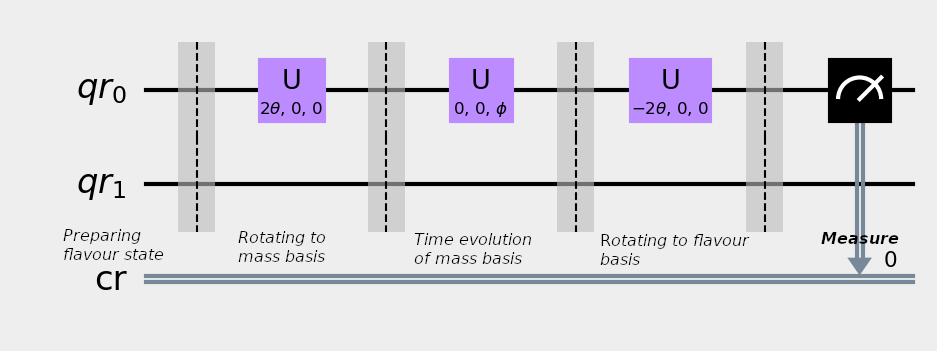
\includegraphics[scale=1]{fig_2.png}}
\caption{Circuit simulating two flavour oscillation\cite{jones}. This is a single qubit circuit utilising only unitary single-qubit gates. }
\label{fig 2}
\end{figure}
\begin{comment}
Thus using a U gate we can realise the PMNS matrix by suitably choosing the value of the parameters. 
\begin{equation}
\label{eq:16}
U_{PMNS}^{2x2} = U(2\theta,0,0) = \begin{bmatrix} cos(\theta) &- \sin(\theta) \\ sin(\theta) & 
cos(\theta) \end{bmatrix}
\end{equation}
Where $\theta$ is the mixing angle and is determined by experimentally.\par

Applying the PMNS matrix that we realised using U gate to flavour state encoded in the qubit $\ref{eq:14}$ we can rotate it into in the mass basis ($\ket{\nu_{1}},\ket{\nu_{2}}$). Then, for witnessing the neutrino oscillation we have to time evolve the mass states. 
\begin{gather*}
\begin{split}
\ket{\nu_{\alpha}(t=0)}& = U_{\alpha 1}\ket{\nu_{1}} + U_{\alpha 2}\ket{\nu_{2}}  \\
\ket{\nu_{\alpha}(t)}& = U_{\alpha 1}e^{i\phi_{1}}\ket{\nu_{1}} + U_{\alpha 2}e^{i\phi_{2}}\ket{\nu_{2}}\\
&=e^{i\phi_{1}}( U_{\alpha 1}\ket{\nu_{1}} + U_{\alpha 2} e^{ i\Delta\phi}\ket{\nu_{2}}
\end{split}
\end{gather*}
Where $\Delta\phi=\phi = \phi_{2}-\phi_{1}$.
Global phases like $e^{i\phi_{1}}$ have no physical significance and can be discarded\cite{benenti}, relative phases between mass states are only relevant for neutrino oscillations, and without losing any generality we can measure all phases relative to $\ket{\nu_{1}}$ state. The time evolution operator can also be encoded by using a U gate.
\begin{equation}
\textbf{U(t)} = U(0,0,\phi) = \begin{bmatrix} 1 & 0 \\ 0 & e^{i\phi} \end{bmatrix}
\end{equation}
Where $\phi = \frac {\Delta m^{2} t}{2E}$ ( refer \ref{eq:6} ,\ref{eq:6a}) in natural units and under ultra relativistic approximation.\par
After time evolving the mass states it is rotated again back into flavour basis by applying $U^{\dagger}$ and is measured to get back the final state. By simply changing parameter $\theta \rightarrow -\theta$ in $\ref{eq:16}$, $U^{\dagger}$ can be encoded using U gate. 
\begin{equation}
U_{PMNS}^{2x2 \ \dagger}= U(-2\theta,0,0) = \begin{bmatrix} cos(\theta) & \sin(\theta) \\ -sin(\theta) & cos(\theta) \end{bmatrix}
\end{equation}

\end{comment}

\section{Simulating three flavour Neutrino Oscillation}\label{3FO}
Using only one qubit we can only construct a Hilbert space of dimension two. A three flavour neutrino oscillation involves a dimension of 3 and requires more than one qubit. So three flavours of neutrino are encoded by using 2 qubits. The encoding scheme we follow is that,
\begin{equation}
\label{eq:17}
\begin{split}
\ket{\nu_{e}}& = \ket{00} = \begin{bmatrix} 1\\0\\0\\0 \end{bmatrix}, \ \ket{\nu_{\tau}} = \ket{01} = \begin{bmatrix} 0\\1\\0\\0 \end{bmatrix} \\
\ket{\nu_{\mu}}&=\ket{10}=\begin{bmatrix} 0\\0\\1\\0 \end{bmatrix}, \ \ket{\nu_{x}} = \ket{01} = \begin{bmatrix} 0\\0\\0\\1 \end{bmatrix} 
\end{split}
\end{equation}
There is one redundant basis state  $\ket{\nu_{x}}$ in this encoding. This could represent the fourth flavour of neutrino in models with sterile neutrinos. But for our discussion, we consider it as physically decoupled and thus unphysical. The circuit is designed in such a way that fourth state does not take part in oscillation. Here also we follow the same methodology as discussed in the two flavour case. We prepare flavour states and do the unitary transformation of flavour state into mass basis, then time evolve the mass states and transform it back into flavour basis and measure it. Realising the PMNS matrix using quantum gates is not trivial as in the case of two flavour case. Here we follow the circuit proposed by Arguelles et.al (2019)\cite{jones}, in which $U$ gates and CNOT gates are used for realising the PMNS matrix. 
\begin{figure}[h]
\graphicspath{ {./Images/} }
\centering	
{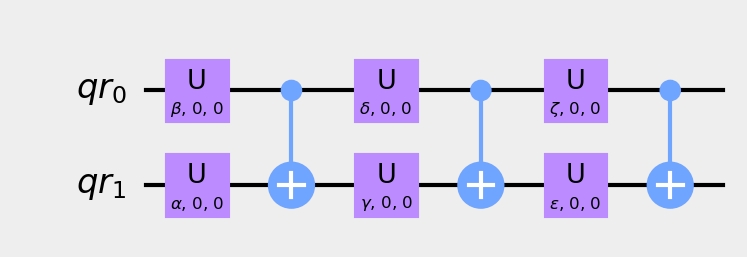
\includegraphics[scale=1]{fig_3.png}}
\caption{Gate arrangement for realizing PMNS matrix\cite{jones}}
\label{fig 3}
\end{figure}

The above circuit is designed in such a way as to mimic the action of the PMNS matrix. To fit the free parameters on this circuit, the circuit is mapped onto a matrix multiplication on the computational basis and perform a numerical fit to match the experimentally determined PMNS matrix. The input values of the PMNS matrix used to fit the parameters are from \cite{estaban} and are,
\begin{equation}
U_{PMNS} = \begin{bmatrix} 0.821427 & 0.550313 & 0.149708 & 0 \\ -0.481513&0.528538&0.699138&0\\0.305618&-0.646377&0.699138&0\\0&0&0&1 \end{bmatrix}
\end{equation}
Here we consider the PMNS matrix of 4X4 form since the encoding scheme uses 2 qubit which forms 4 dimensional Hilbert space.  The last row represents decoupled physical state and will not take part in flavour oscillation. \par
The PMNS matrix is fitted by the method of gradient minimization over the six parameters (sum of squared residuals of each element of the matrix is minimised). The best fit parameter provided in \cite{jones} are, 
\begin{equation}
\label{eq:18}
\alpha = -0.6031,\ \beta = -2.0125, \ \gamma = -0.7966, \ \delta = 1.0139 ,\  \epsilon = 0.7053, \ \zeta = 1.3599
\end{equation}

Substitution of parameters given by $\ref{eq:18}$ in the circuit would give us PMNS matrix and PMNS$^{\dagger}$ is got by inverting the gate arrangement.\par
The evolution operation $\textbf{U(t)}$ in computational basis is given by,
\begin{equation}
\textbf{U(t)}=\exp [i \ diag(0,\Delta m_{12}^{2}\frac{t}{2E}, \Delta m_{13}^{2}\frac{t}{2E},\Phi)]
\end{equation}
Where $\Phi$ is arbitrary phase that can be picked up for convenience and can be discarded since fourth basis state is not observable. Such a time evolution operator is realised using two $U$ gates.
\begin{equation}
\textbf{U(t)}= U(0,0,\phi_{1})) \otimes U(0,0,\phi_{2})
\end{equation}
Where $\phi_{1}=\frac{\Delta m_{13}^{2}}{2E}$ and $\phi_{2}=\frac{\Delta m_{12}^{2}}{2E}$.\par
The circuit for simulating three flavour oscillation is given below.
\begin{figure}[h]
\graphicspath{ {./Images/} }
\centering	
{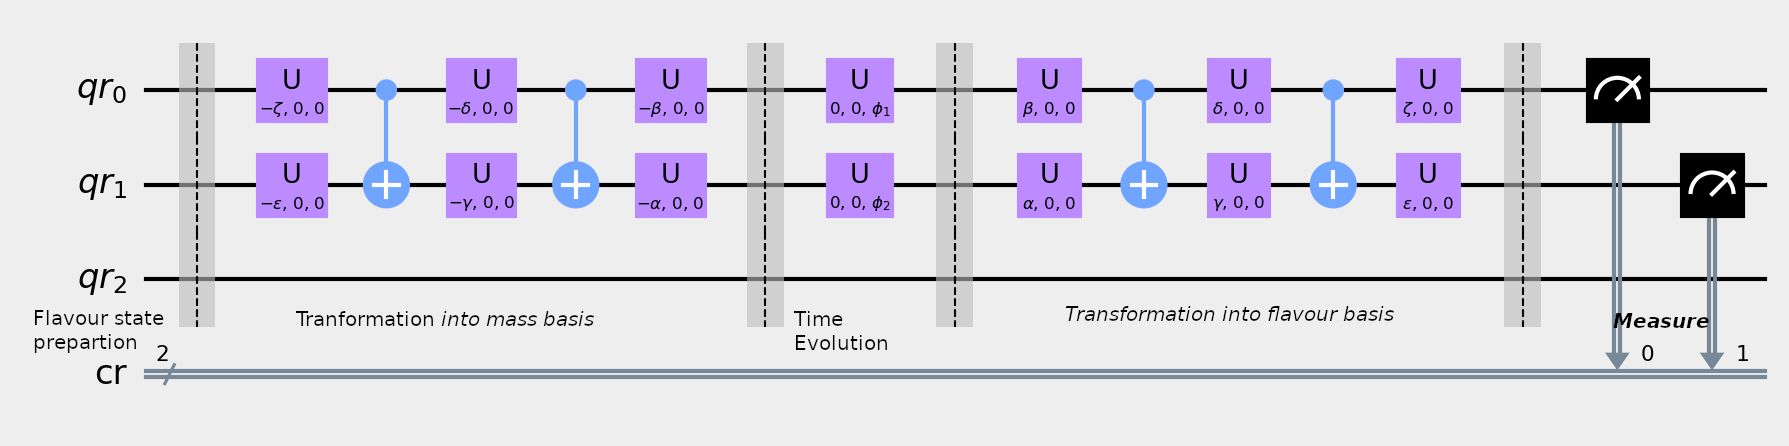
\includegraphics[scale=0.5]{fig_4.png}}
\caption{Circuit for simulating three flavour oscillation\cite{jones}. Circuit can be repeatedly run to prepare qubits in the flavour state, time evolve them and measure them in the flavour basis.}
\label{fig 4}
\end{figure}

It should be noted that, this circuit is complex compared to two flavour case, read out errors and gate error will be more compared to the former. Also this circuit can be also extended to incorporate sterile neutrinos and to study matter effects(MSW effects). Scheme for such studies are also provided in \cite{jones}.
\newpage
\thispagestyle{empty}
\mbox{}
\newpage
\chapter{Simulation Results}
We used IBM Quantum Experience which is a cloud-based computing service provided by IBM to run our circuits. IBM Q ( short form of IBM Quantum Experience) provides about 26 quantum services which comprise of 5 different types of simulators (including QASM Simulator) and 21 Quantum computers. Out of the 21 Quantum Computers, 8 are publicly accessible and the remaining are exclusive for the collaborators. Even though great advancement has been made in this field over the decade, still technology remains imperfect. Each gate applied to the circuit would induce an error of $\mathcal{O}(0.1\%)$ and per qubit readout error of $\mathcal{O}(5\%)$. Thus the error in the result increases as the length of the circuit, prohibiting lengthy calculations. But one can employ methods like quantum state tomography or use quantum error-correcting codes to mitigate the errors. 
\section{Two flavour oscillations : Simulation Results} 
With the quantum circuit defined in the section $\ref{2FO}$, we simulated an electron neutrino ($\nu_{e}$) disappearance experiment with the parameters given by the KamLAND experiment \cite{Eugichi}. Kamioka Liquid Scintillator Antineutrino Detector(KamLAND) is an electron antineutrino detector located in the Kamioka observatory. It studies neutrino oscillation using electron antineutrino produced by nuclear reactors.\cite{Iwamoto}.\par
We run 1024 trails and measure the count of output flavour and then calculate the appearance probability from it. Using the QASM simulator circuit performed extremely well and predicted probability that agrees with the theoretical value. We performed simulations for different values of neutrino beam energy while fixing the L to be constant. We plotted how disappearance probability varies as a function of Energy in MeV. It should be noted that we had chosen L=180 KM in order to match the experimental conditions of the KamLAND. 
\begin{figure}[h]
	\graphicspath{ {./Images/} }
	\centering	
	{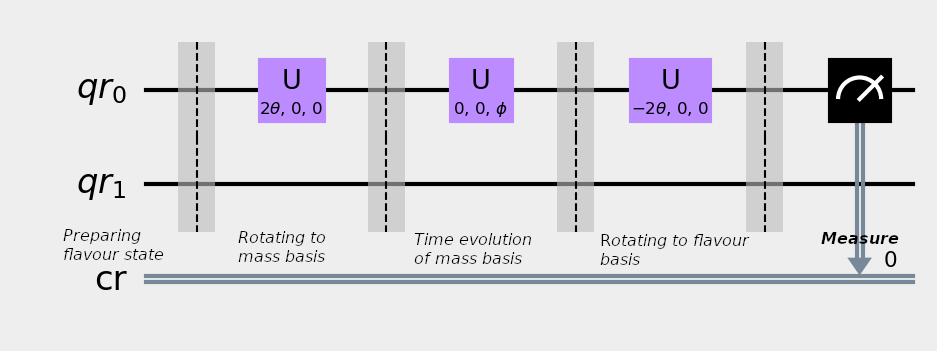
\includegraphics[width=\textwidth]{fig_2.png}}
	\caption{}
	\label{fig 2}
\end{figure}\par
Electron neutrino state is encoded into $\ket{0}$ state. We run 1024 trails and got back the neutrino state after time evolution. From this count, disapperance probability of neutrino was calculated. The experiment was repeated for a range of neutrino beam energies and curve showing how disapperance probability varies with energy was plotted.
\begin{figure}[H]
	\graphicspath{ {./Images/} }
	\centering	
	{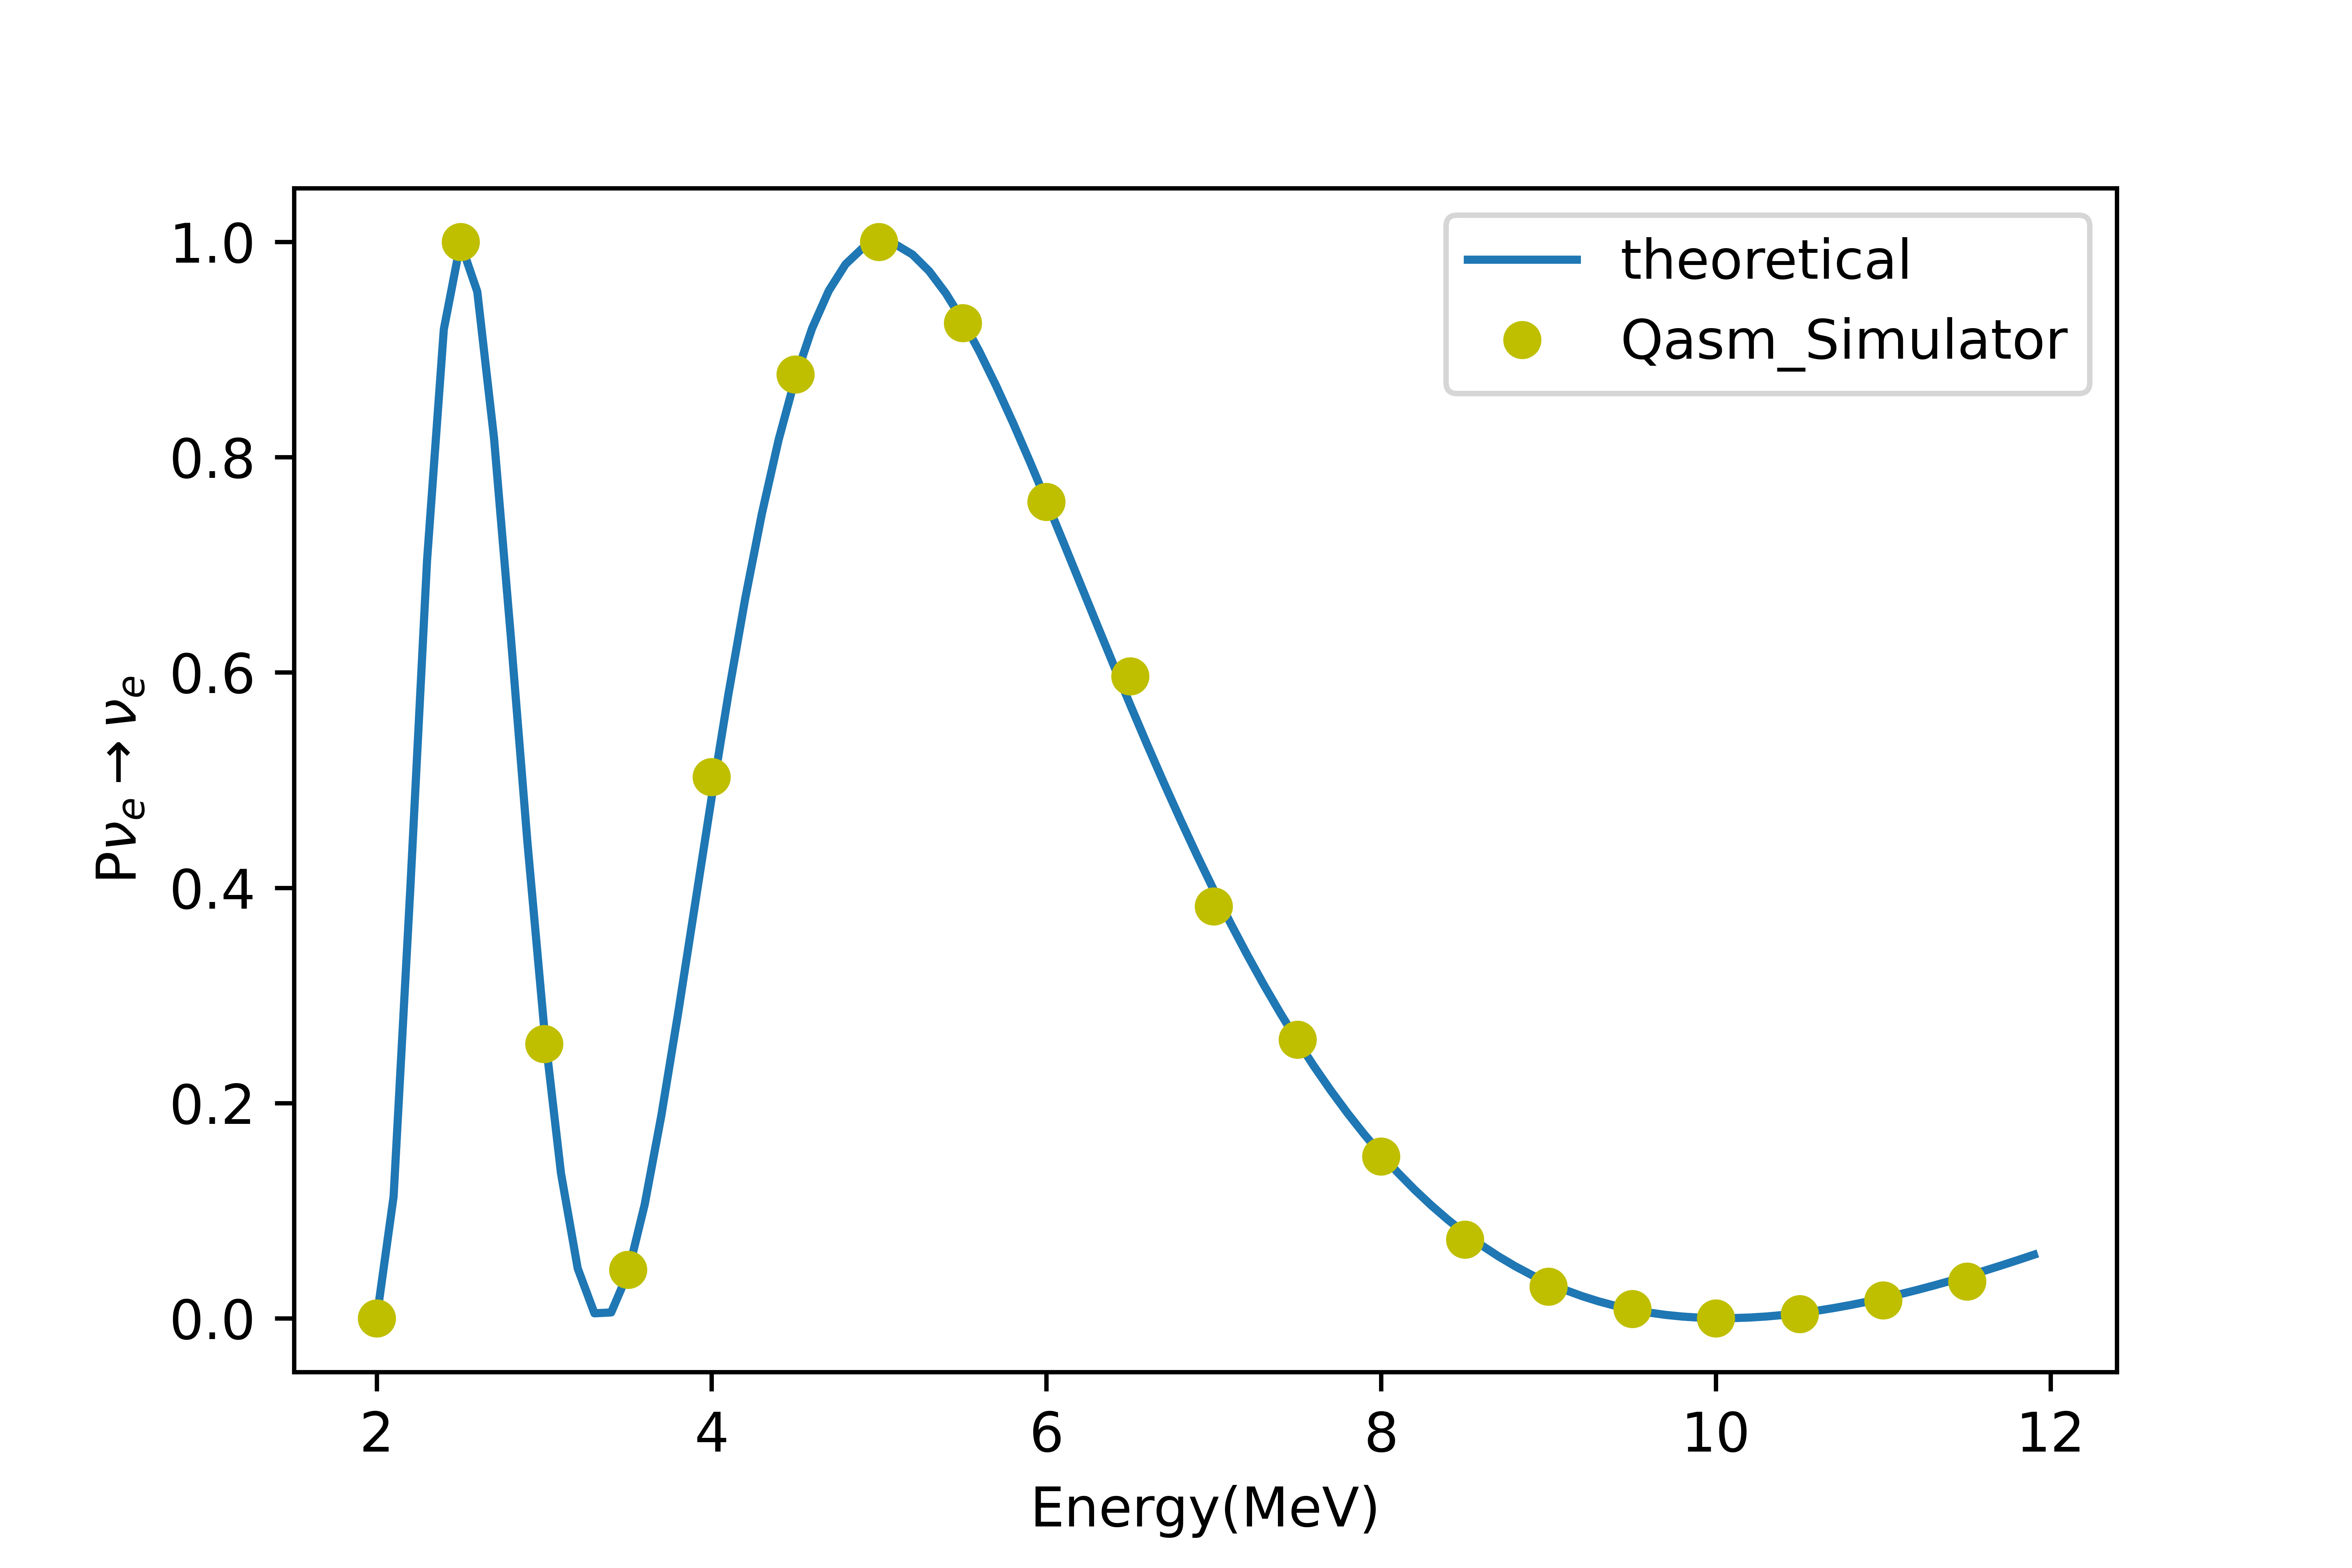
\includegraphics[width=\textwidth]{fig_5.png}}
	\caption{Energy in MeV is plotted in X axis and disappearance probability along Y axis. We observed variation of disappearance probability with energy exhibiting a sinusoidal nature.  }
	\label{fig 5}
\end{figure}\par
From the figure $\ref*{fig 5}$ it is evident that our circuit performs very well and correctly predicts the disappearance probability.
\subsection{Simulating in IBM Quantum Computer}
Circuit provided in figure $\ref*{fig 2}$ is used to perform simulation in IBM Quantum computers. We performed the simulation on a IBM quantum computer named as IBM Armonk. It is a single qubit quantum computer which also supports pulse mode. Like the former we run the circuit 1024 shots and found out neutrino counts. Using this counts calculated the disapperance probability. 
\begin{figure}[H]
	\graphicspath{ {./Images/} }
	\centering	
	{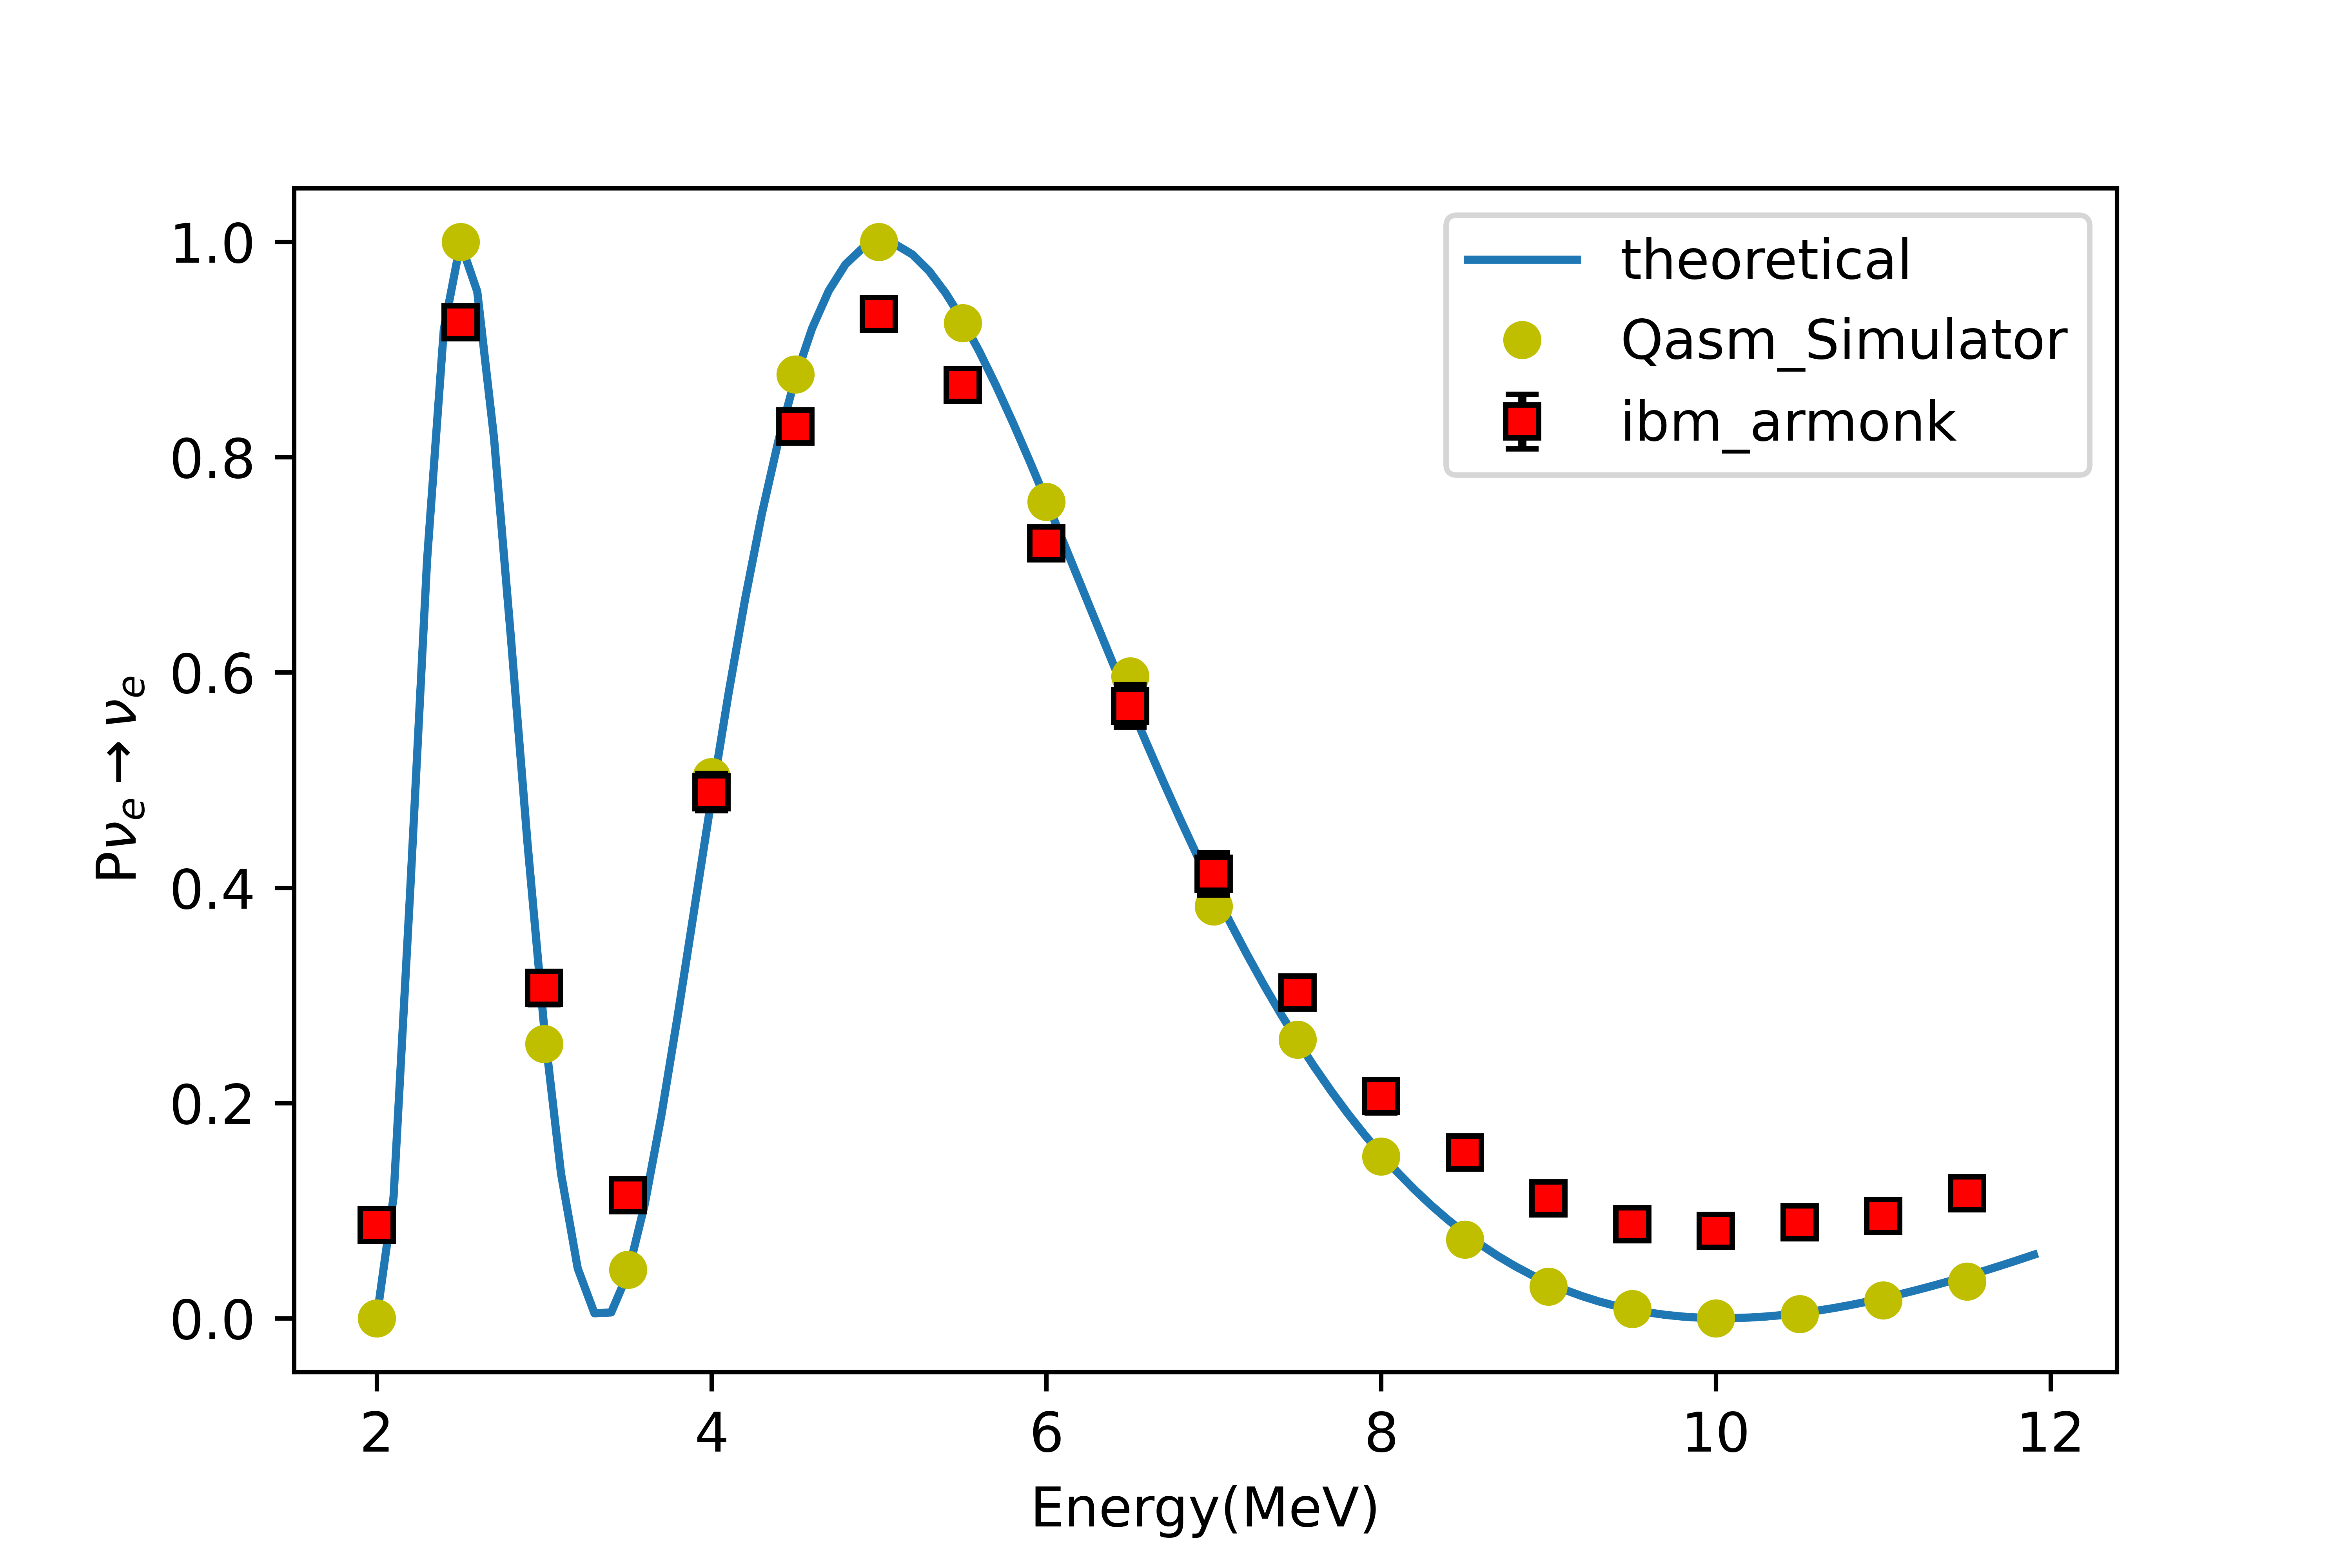
\includegraphics[width=\textwidth]{fig_6.png}}
	\caption{Energy in MeV is plotted in X axis and disappearance probability along Y axis. We observed variation of disappearance probability with energy exhibiting a sinusoidal nature.}
	\label{fig 6}
\end{figure}\par
Here we also have account for the statstical error that may can happen while running circuits on actual quantum computers. For a particular value of energy we repeated the experiment for 10 times and calculated standard deviations of data. From figure $\ref*{fig 6}$ it is evident that the behaviour of theoretical curve by simulational results even though there is error in value predicted by the circuit.

\subsection{Three flavour oscillation: Simulation Results}
Using the circuit shown in the figure $\ref*{fig 4}$ we performed simulations of appearance and disappearance experiment of neutrino beam of muon flavour initially. Parameters required for simulation ( mixing angle and mass square splittings) are taken from \cite{estaban}. From simulations, we calculated the appearance probability of electron and tau neutrinos and also the disappearance probability of muon neutrinos. Simulations were run on both the QASM simulator and the IBM Quantum computer.
\begin{figure}[H]
\graphicspath{ {./Images/} }
\centering	
{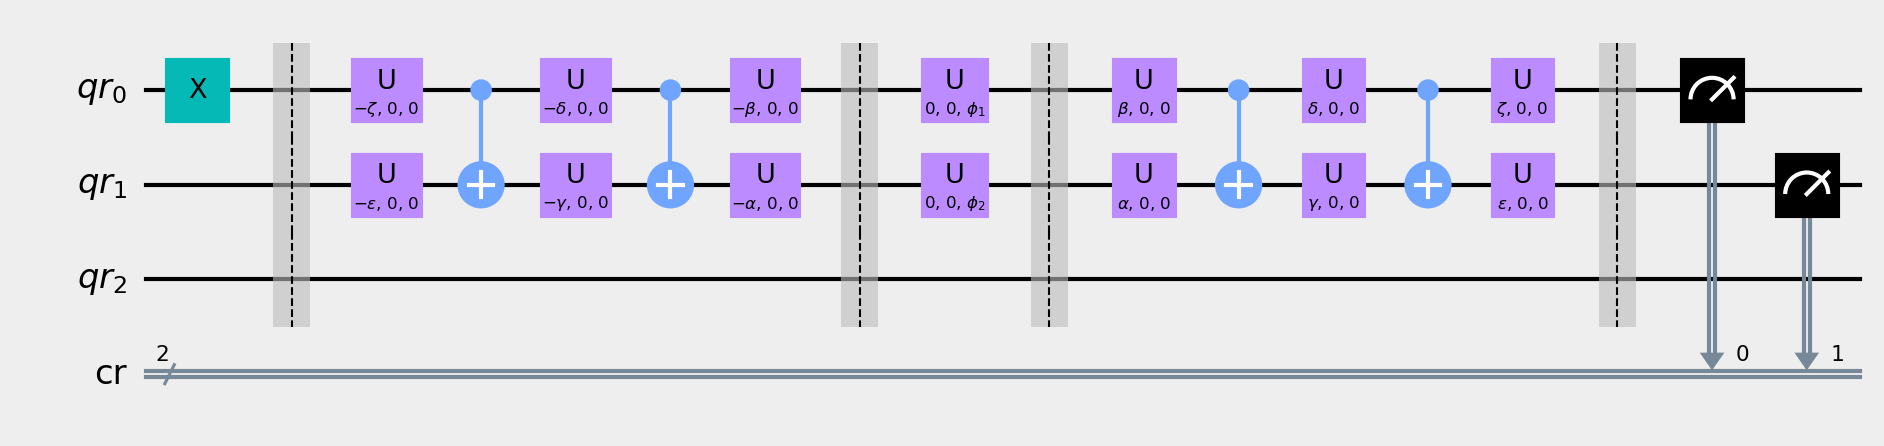
\includegraphics[width=\textwidth]{fig_7.png}}
\caption{Three-flavour oscillation experiment as run on QASM simulator and on the IBM quantum computer}
\label{fig 7}
\end{figure}\par
Here we initially prepare muon neutrino as per the encoding scheme discussed earlier ( refer equation $\ref{eq:17}$), them time evolve it and measure the final state of neutrino.
\subsection{Simulating in QASM Simulator}
We calculated disappearance probability muon and appearance probability of electron and tau for various values $\frac{L}{E}$ with each experiment composed of 1024 trials. The plot showing how probabilities vary with $\frac{L}{E}$ is plotted.

From the figure $\ref*{fig 8}$ it is clear that circuit works fine even though there are slight deviations can from theoretical value. The oscillation probabilites given by the circuit retains the sinusoidal nature as predicted by the theory.
\begin{figure}[H]
	\graphicspath{ {./Images/} }	
	{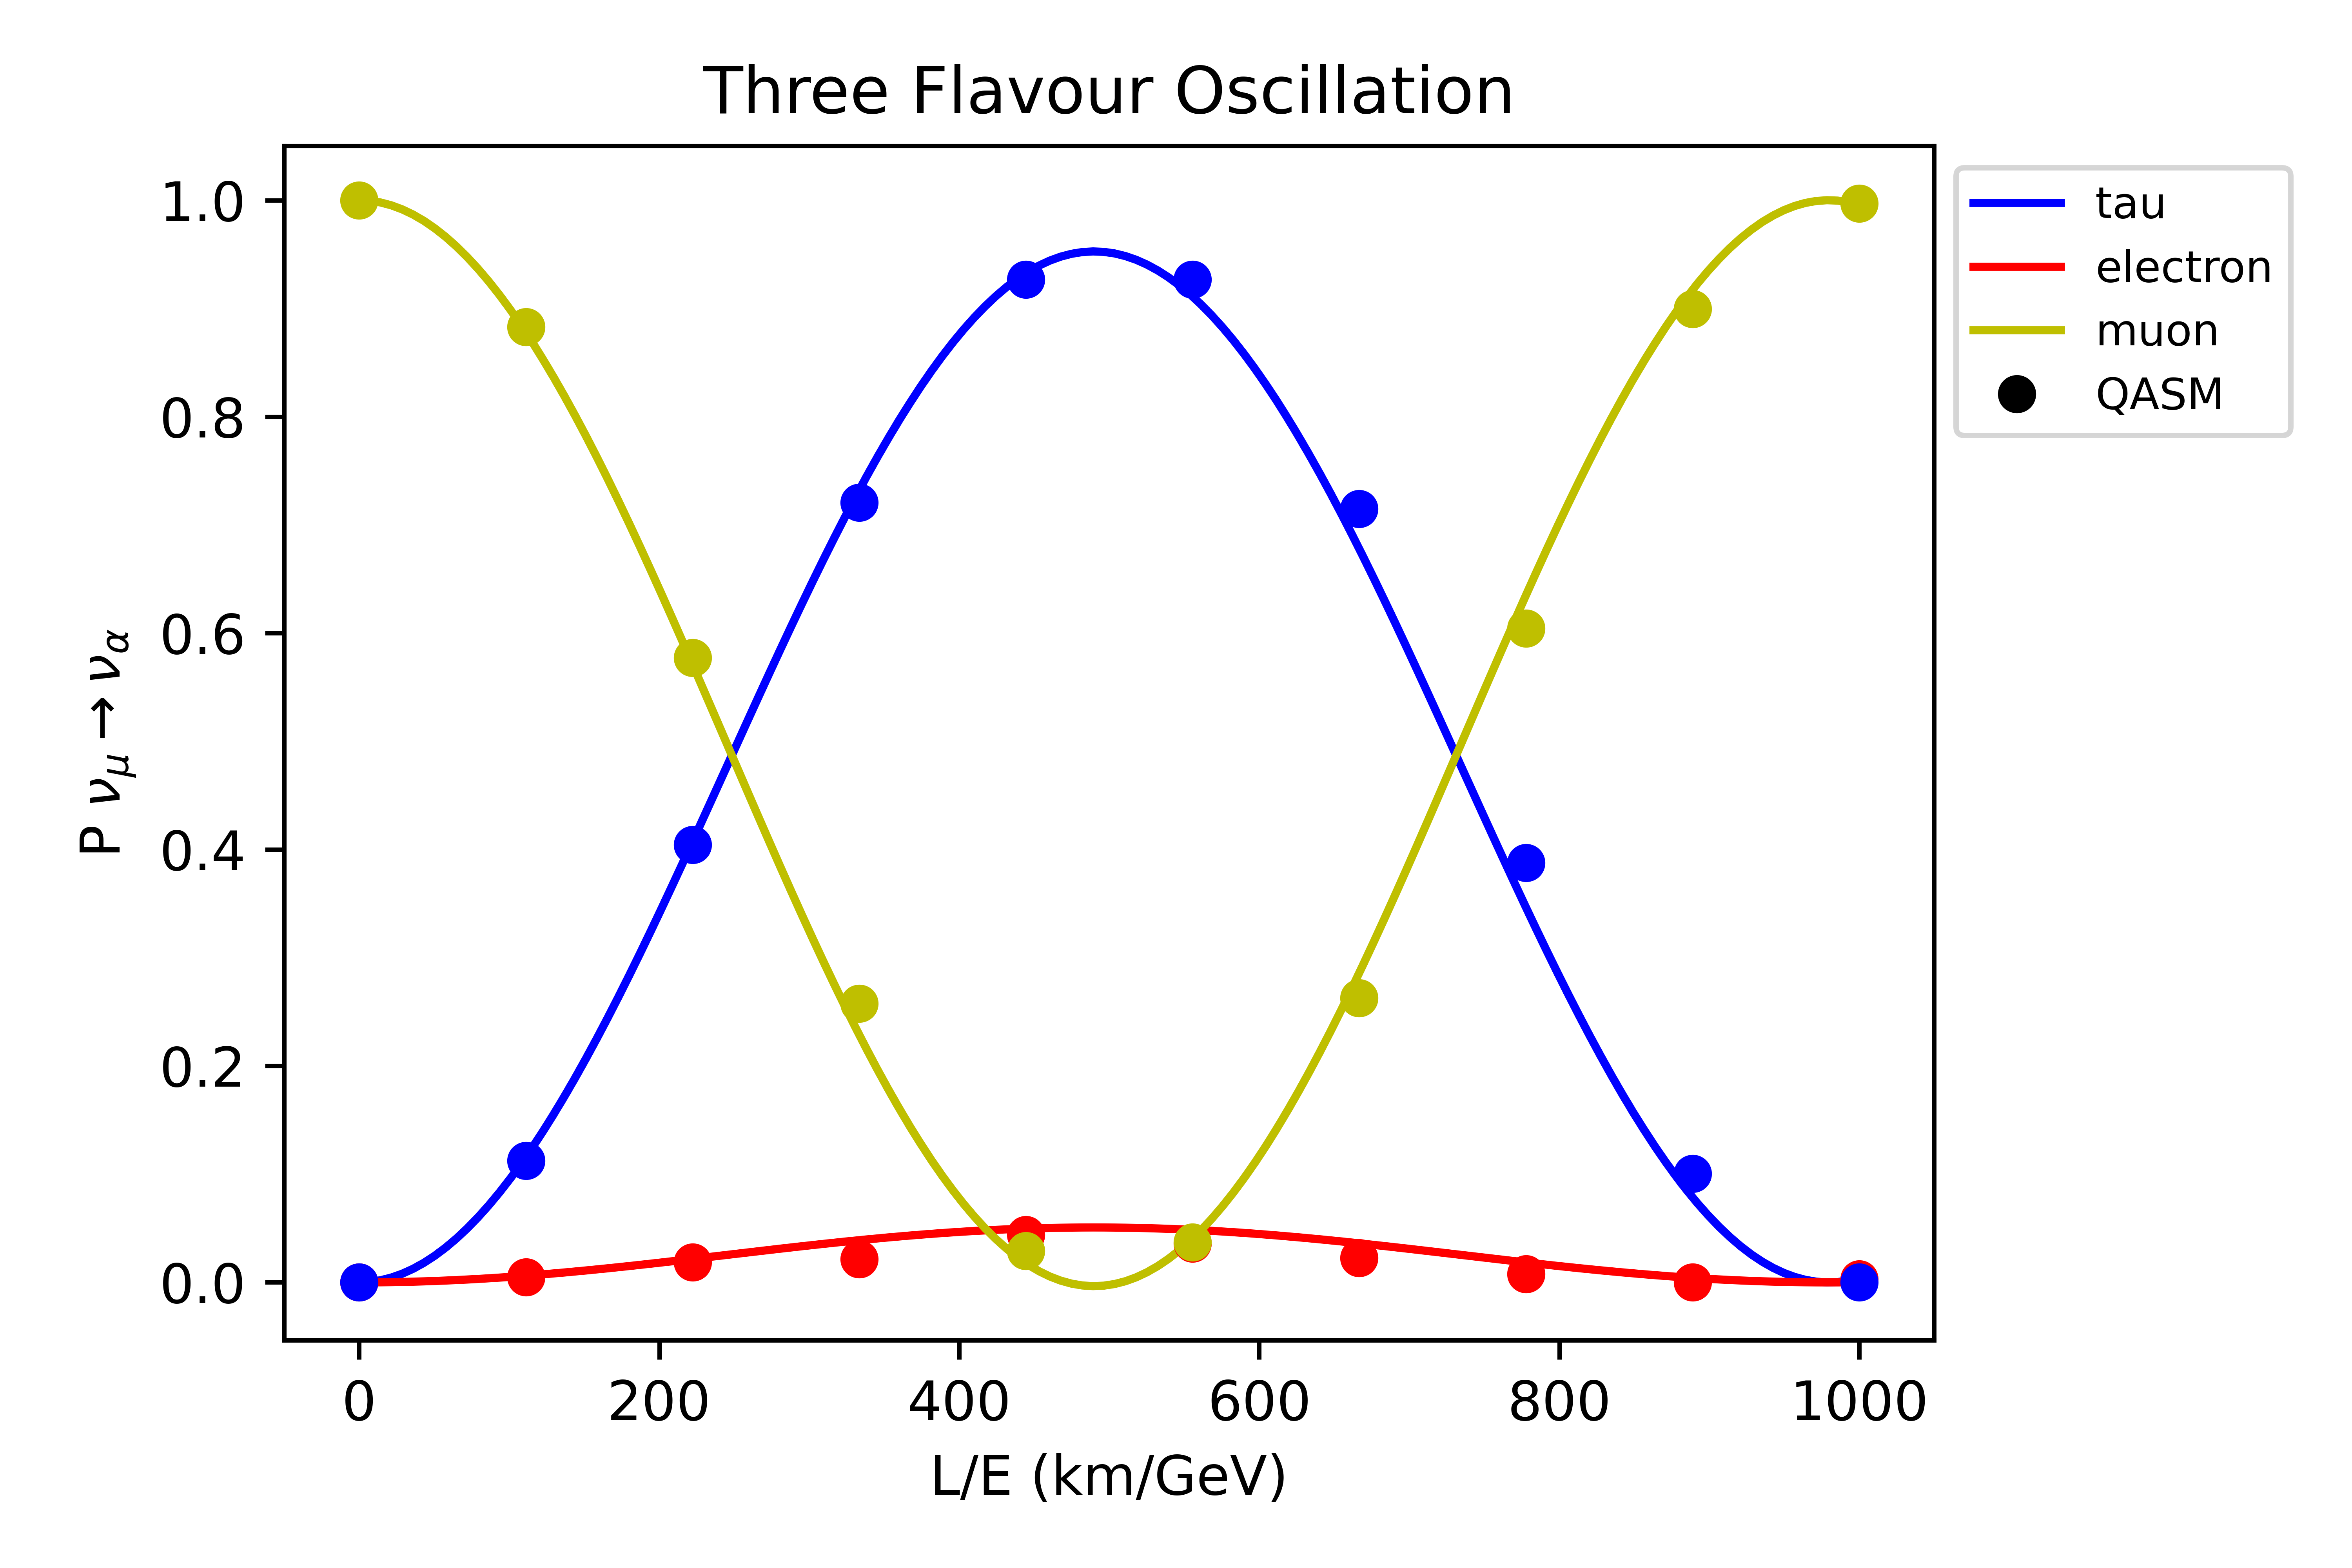
\includegraphics[width=\textwidth]{fig_8.png}}
	\centering\caption{ Oscillation probability is plotted in y axis and $\frac{L}{E}$ ( $\frac{KM}{GeV}$) along x axis. It should be noted that $\alpha$ represent an arbitrary flavour state and can be electron, muon or tau.}
		\label{fig 8}
	\end{figure}

\subsection{Simulating In Quantum computer}
The circuit was run on IBM Quantum computer named IBM Lima. We run the circuit 1024 shots and from it found the final neutrino counts. Oscillation probabilities were founded from these counts and experiment was repeated for different $\frac{L}{E}$ values.
\begin{figure}[h]
	\graphicspath{ {./Images/} }
	\centering	
	{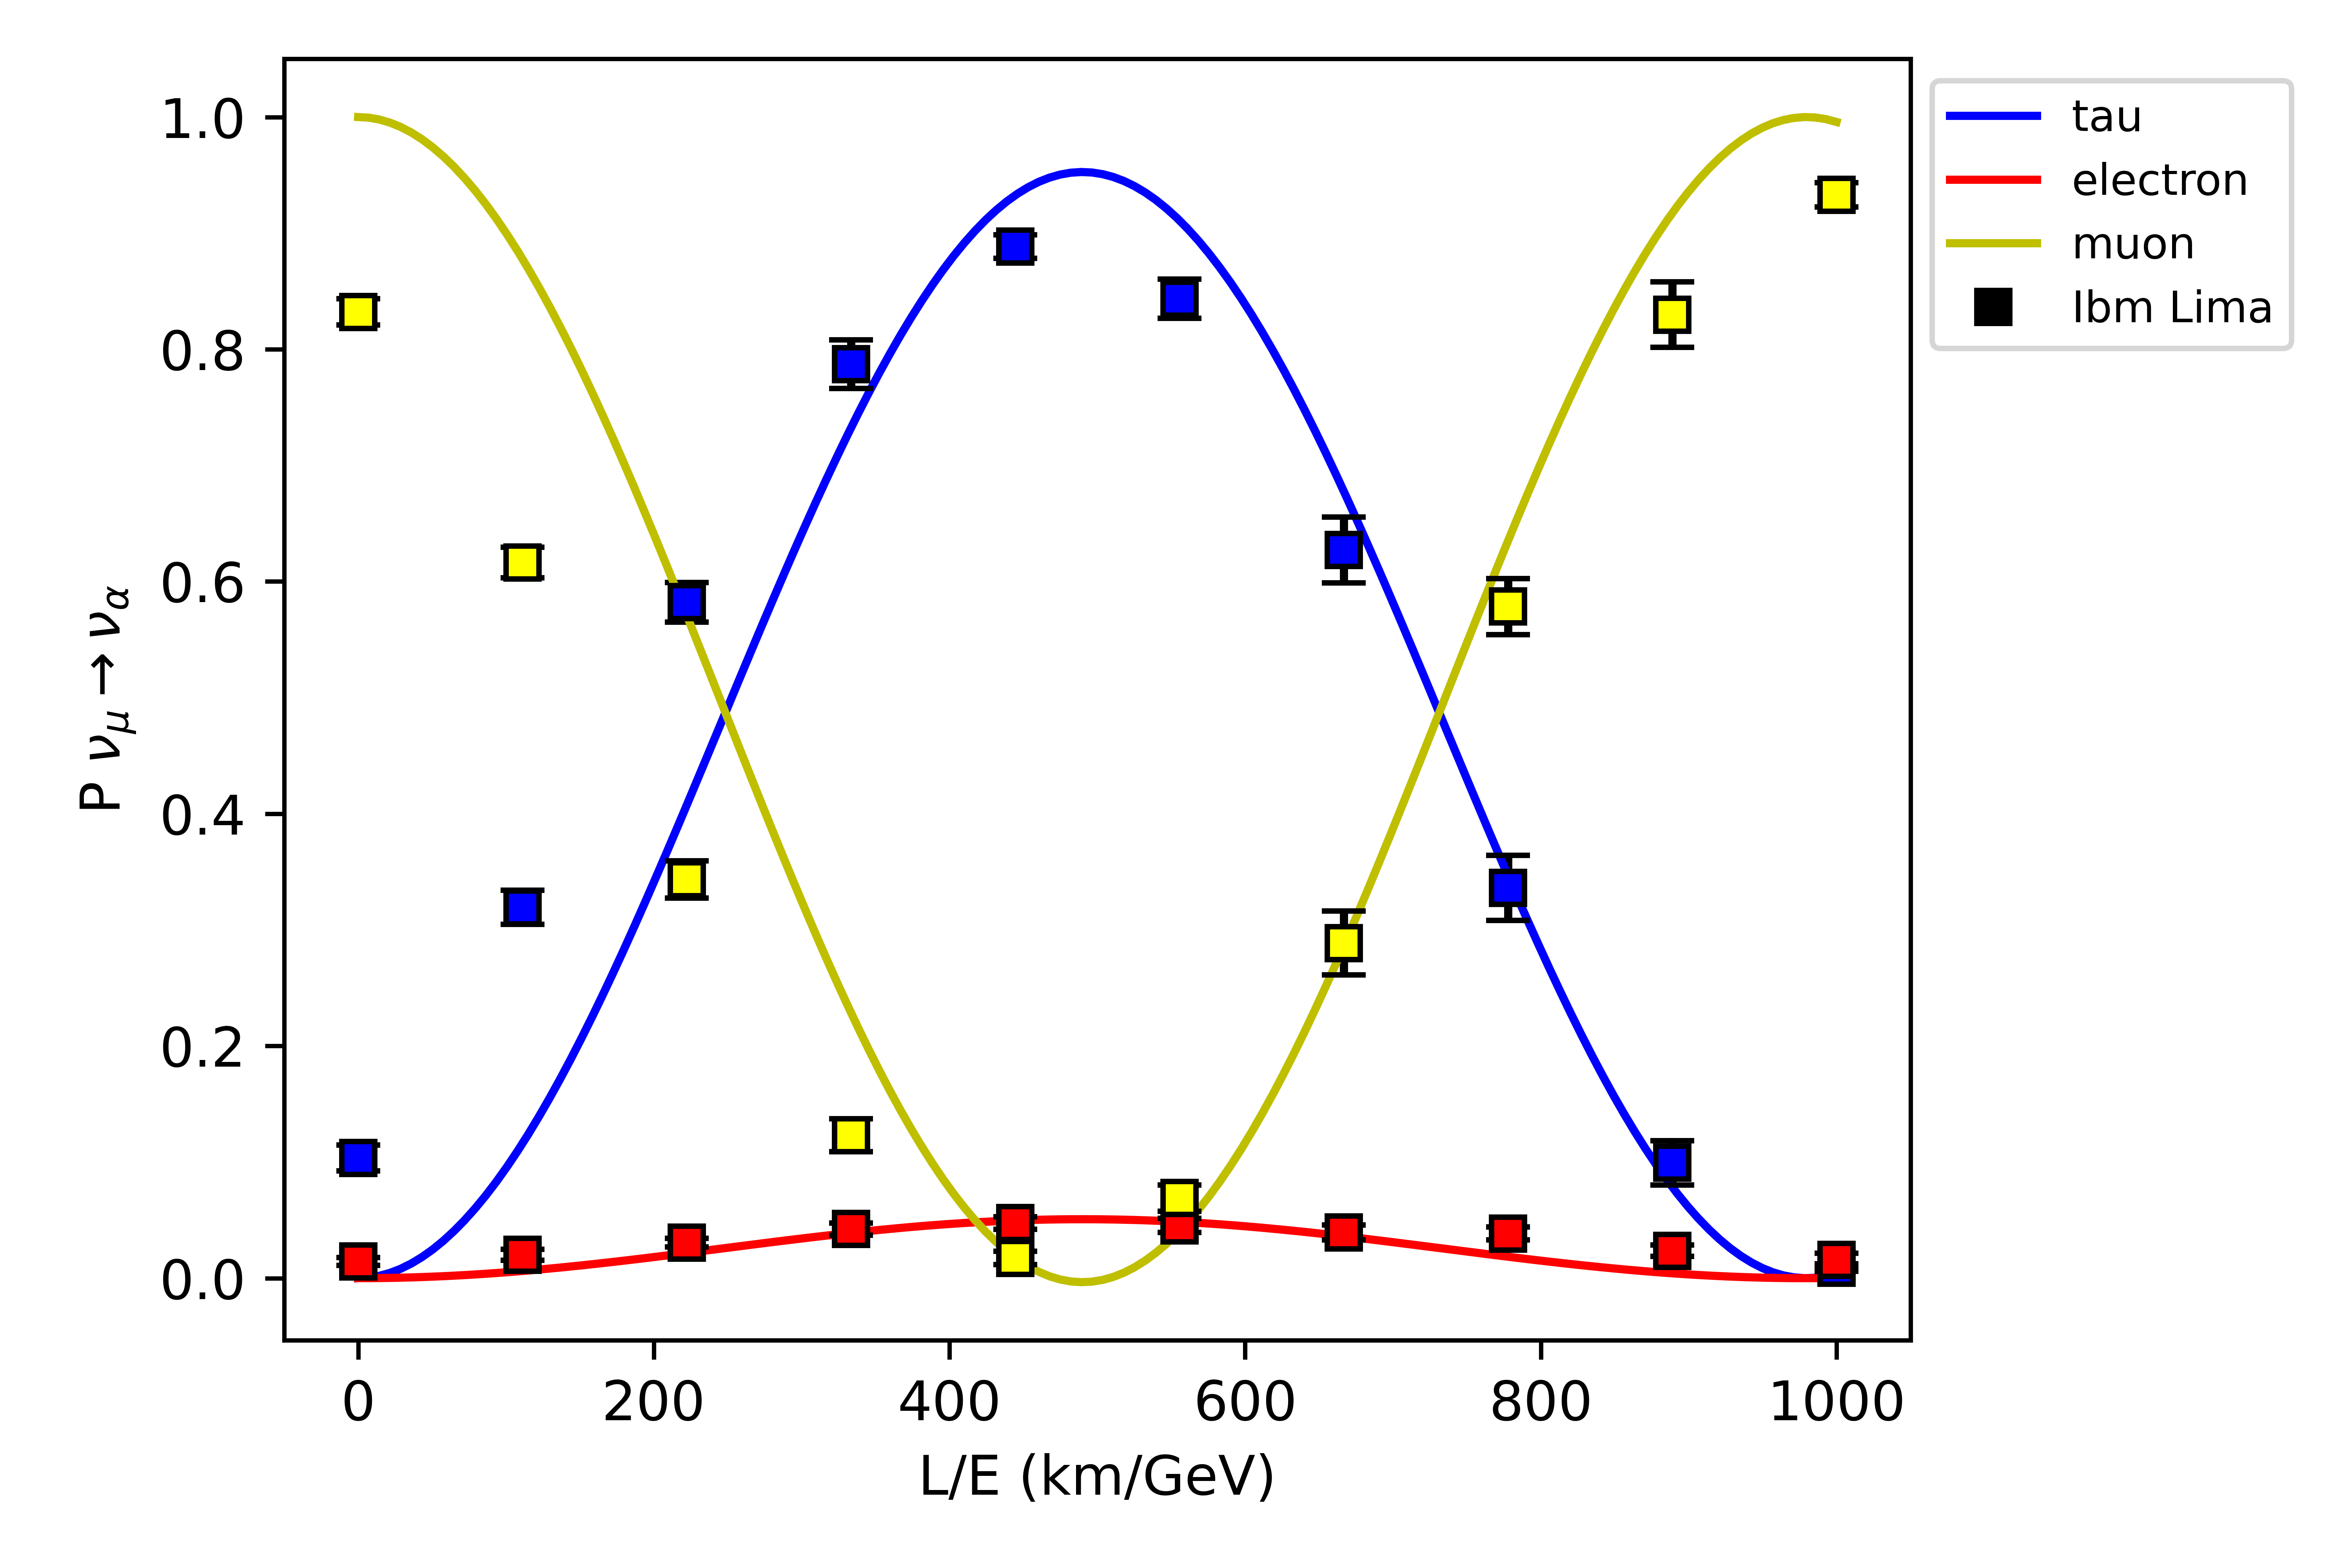
\includegraphics[width=\textwidth]{fig_9.png}}
	\caption{$\frac{L}{E}$ ( $\frac{KM}{MeV}$) is plotted in X axis and Probability along y axis. $\alpha$ can be electron, muon or tau.}
		\label{fig 9}
	\end{figure}
	Here we also have accounted for the statistical error that may happen while running circuits on actual quantum computers. For a particular value of $\frac{L}{E}$, we repeated the experiment 10 times and calculated standard deviations of data. \par 
	One can see deviations of oscillation probabilities predicted by the circuit from the actual value. As discussed above, the errors are due large length of the circuit. Compared to two flavour case, number single qubit gates used is 5 times large and each gate approximately induce an error of $\mathcal{O}(0.1\%)$ . Additionally this circuit uses 4 two qubit gates which also induce errors into results. Further readout errors  ($\mathcal{O}(5\%)$ can also influence final results.
	
\bibliography{ref}
\printindex

\end{document}
